\section{Regresión: Análisis Estadístico de Datos}

\subsection{Introducción}

Para el problema de regresión hacemos uso del dataset \textbf{autoMPG6} \cite{autompg}, donde se codifica el consumo de gasolina de distintos coches (en millas por galón, Mpg) en base a las siguientes características:

\begin{enumerate}
\def\labelenumi{\arabic{enumi}.}
    \item \textbf{Displacement}: Indica la cilindrada del coche, la suma del volumen útil de los cilindros del motor, medido en pulgadas cúbicas.
    \item \textbf{Horse\_power}: Mide la potencia del coche.
    \item \textbf{Weight}: Peso en libras.
    \item \textbf{Acceleration}: Aceleración del coche de 0 a 60 millas por hora, medido
    en segundos.
    \item \textbf{Model\_year}: Indica las dos últimas cifras del año de producción.
\end{enumerate}

El objetivo es poder predecir con estos cinco atributos el consumo de Mpg de un nuevo coche:

\begin{enumerate}
    \def\labelenumi{\arabic{enumi}.}
    \setcounter{enumi}{5}
    \item \textbf{Mpg}: Millas-por-galón, indica la cantidad de galones (1G $\approx$ 3,78L) de fuél que consume un vehículo al recorrer una milla (1m $\approx$ 1,6km).
\end{enumerate}

El dataset contiene 392 instancias codificando esta información.

\vspace{\baselineskip}

La descripción del problema nos da alguna información adicional sobre las variables:

\begin{enumerate}
    \def\labelenumi{\arabic{enumi}.}
    \item \textbf{Displacement}: Variable numérica continua, contamos con valores reales en el rango {[}68.0,455.0{]}.
    \item \textbf{Horse\_power}: Variable numérica continua, contamos con valores enteros en el rango {[}46,230{]}.
    \item \textbf{Weight}: Variable numérica continua, contamos con valores enteros en el rango {[}1613,5140{]}.
    \item \textbf{Acceleration}: Variable numérica continua, contamos con valores reales en el rango {[}8.0,24.8{]}.
    \item \textbf{Model\_year}: Variable numérica discreta, contamos con valores enteros en el rango {[}70,82{]}.
    \item \textbf{Mpg}: Variable numérica continua, contamos con valores reales en el rango {[}9.0,46.6{]}.
\end{enumerate}

\paragraph{Hipótesis de partida}

\begin{itemize}
    \item \textbf{H.1}: Horse\_power puede influir en Mpg: A más potencia, más consumo.
    \item \textbf{H.2}: Weight debe influir en Mpg: Un coche más pesado debería consumir más.
    \item \textbf{H.3}: Debería haber correlación entre displacement (cilindrada) con horse y acceleration
    \item \textbf{H.4}: Horse y acceleration podrían estar relacionadas
    \item \textbf{H.5}: Viendo que contamos con un rango pequeño de años, no debería haber un cambio significativo de prestaciones entre años
    \item \textbf{H.6}: Pero debería existir una tendencia de mejora de prestaciones con los años, incluyendo aumento de Displacement, Horse\_power y Acceleration.
    \item \textbf{H.7}: Model\_year podría no mostrar relación con Mpg: Pese al paso de los años si contamos con diferentes tipos de vehículos (todoterrenos, familiares, deportivos\ldots) podría haber un consumo dispar. (Si existiera tendencia, viendo que los años son de las últimas décadas del siglo XX, podría ir el consumo hacia abajo)
    \item \textbf{H.8}: Esta última hipótesis se puede aplicar al resto de variables, indicándonos que Model\_year no debería tener relevancia para este problema de regresión.
    \item \textbf{H.9}: Horse\_power podría depender de las variables Displacement y Weight
\end{itemize}

\subsection{Análisis Estadístico de Datos}

Antes de comenzar a analizar las variables nos plantemos una cuestión: ¿Debemos considerar Model\_year como una variable numérica o como un factor categórico? Aunque por la hipótesis H.7 podríamos acabar no eligiendo la variable para el problema, es necesario preguntarnos por esto antes de comenzar.

\vspace{\baselineskip}

Sabemos que las observaciones para esta variable cuenta con valores entre 72 y 82, por lo que tenemos información exacta del año (en comparación, por ejemplo, con agrupaciones mayores como la década o el siglo). El hecho de tratarla como categórica o cuantitativa depende mucho del problema. En este caso, tenemos interés en cuestionarnos por valores entre años, por ejemplo, el consumo entre los años 75 y 76.

\vspace{\baselineskip}

Por tanto, de cara al problema de regresión que nos atañe, tendríamos dos opciones: 
\begin{itemize}
    \item Mantenerlo como categórico y generar variables dummy (valores 0-1 para indicar si la instancia es de ese año). Suponiendo que tenemos al menos una instancia de cada año, esto nos generaría 12 variables nuevas. 
    \item Mantenerlo como numérico, pero teniendo cuidado de cómo interpretar el año.
\end{itemize}

\vspace{\baselineskip}

Proseguimos con tanto dejando Model\_year como variable numérica.

\subsubsection{Análisis univariable}
  
La cabecera de nuestro dataset tiene esta forma:

\begin{tabular}{|r|r|r|r|r|r|}
    \hline
    Displacement & Horse\_power & Weight & Acceleration & Model\_year & Mpg\\
    \hline
    91 & 70 & 1955 & 20.5 & 71 & 26.0\\
    \hline
    232 & 100 & 2789 & 15.0 & 73 & 18.0\\
    \hline
    350 & 145 & 4055 & 12.0 & 76 & 13.0\\
    \hline
    318 & 140 & 4080 & 13.7 & 78 & 17.5\\
    \hline
    113 & 95 & 2372 & 15.0 & 70 & 24.0\\
    \hline
    97 & 60 & 1834 & 19.0 & 71 & 27.0\\
    \hline
\end{tabular}

\vspace{\baselineskip}

Y con la siguiente información estadística:

\begin{verbatim}
  Displacement    Horse_power        Weight      Acceleration     Model_year   
 Min.   : 68.0   Min.   : 46.0   Min.   :1613   Min.   : 8.00   Min.   :70.00  
 1st Qu.:105.0   1st Qu.: 75.0   1st Qu.:2225   1st Qu.:13.78   1st Qu.:73.00  
 Median :151.0   Median : 93.5   Median :2804   Median :15.50   Median :76.00  
 Mean   :194.4   Mean   :104.5   Mean   :2978   Mean   :15.54   Mean   :75.98  
 3rd Qu.:275.8   3rd Qu.:126.0   3rd Qu.:3615   3rd Qu.:17.02   3rd Qu.:79.00  
 Max.   :455.0   Max.   :230.0   Max.   :5140   Max.   :24.80   Max.   :82.00  
      Mpg       
 Min.   : 9.00  
 1st Qu.:17.00  
 Median :22.75  
 Mean   :23.45  
 3rd Qu.:29.00  
 Max.   :46.60  
\end{verbatim}

\vspace{\baselineskip}

El dataset \textbf{no} cuenta con \textbf{valores repetidos} ni \textbf{missing values}.

\vspace{\baselineskip}


% \begin{figure}[H]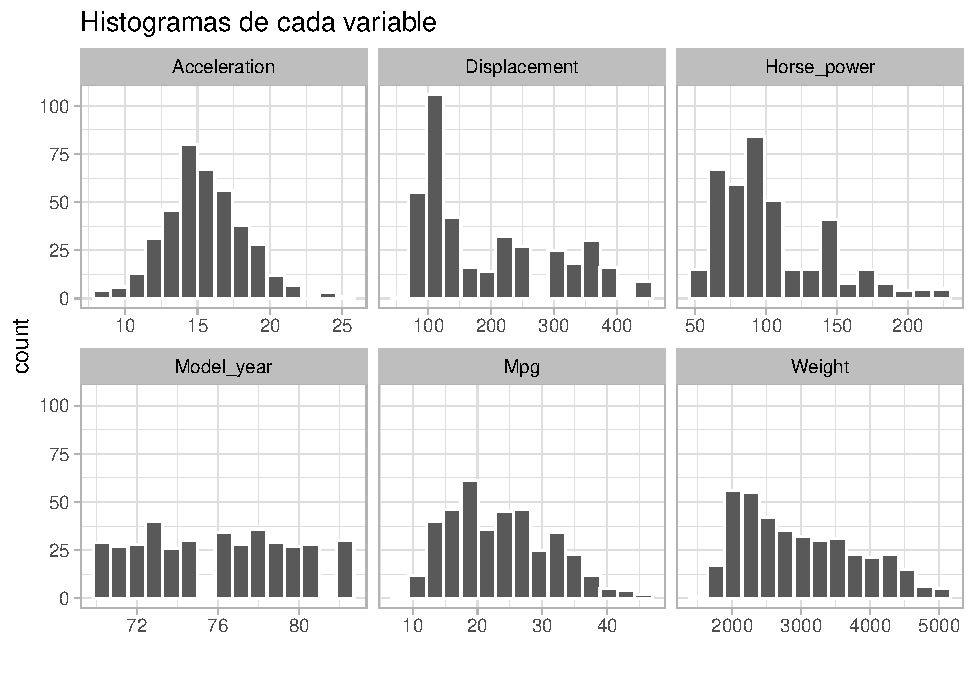
\includegraphics[width=.9\linewidth]{img/EDA_files/figure-latex/unnamed-chunk-6-1} \caption{}\end{figure}

% Una a una

Mostramos scatterplots univariables:
\begin{figure}[H]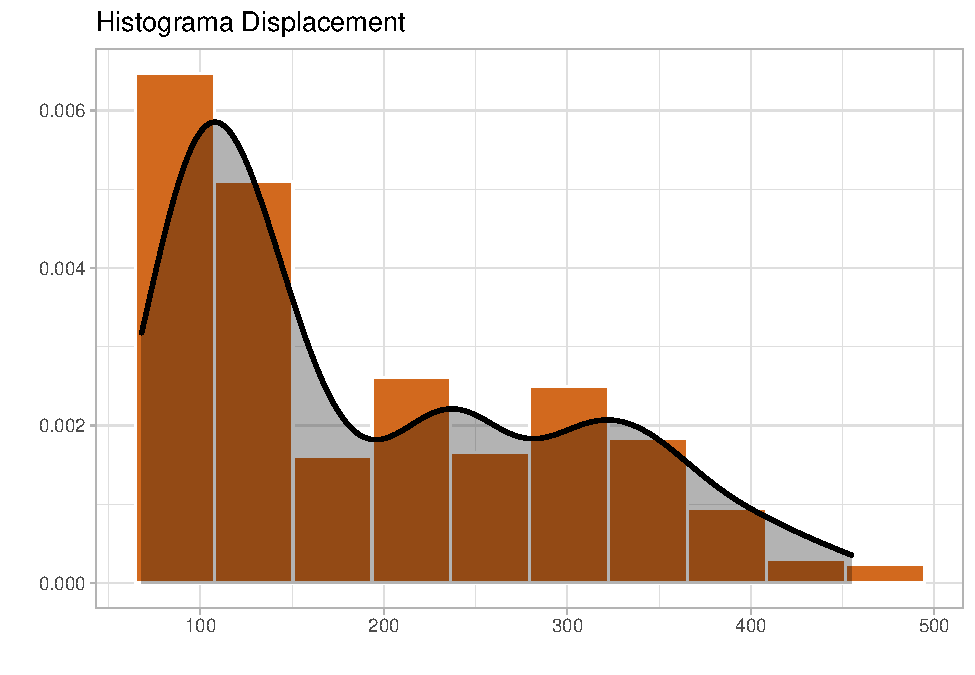
\includegraphics[width=.9\linewidth]{img/EDA_files/figure-latex/unnamed-chunk-7-1}\caption{}\end{figure}
\begin{figure}[H]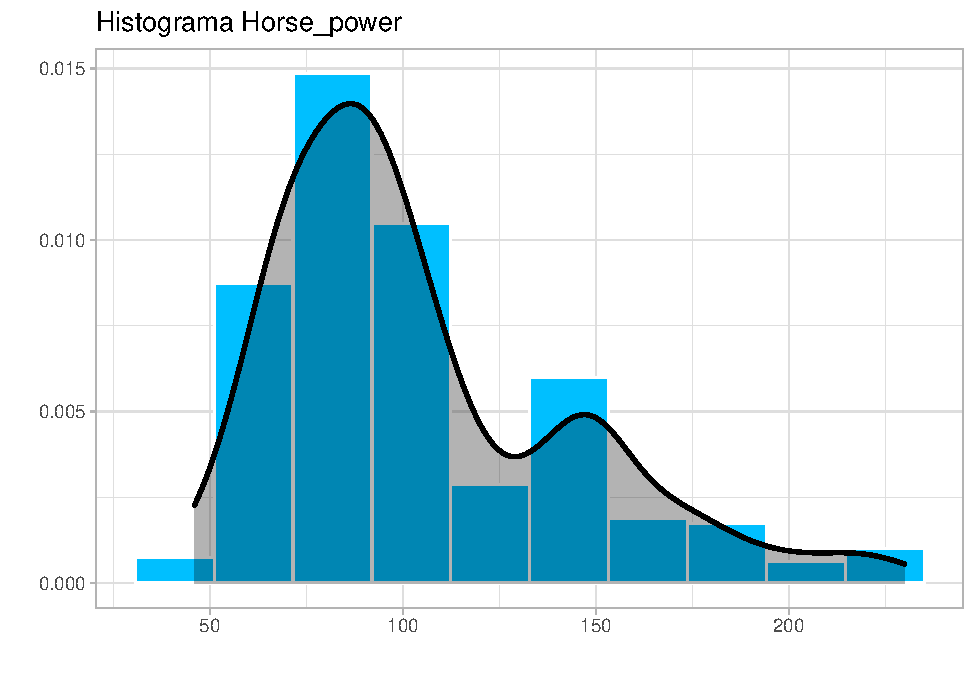
\includegraphics[width=.9\linewidth]{img/EDA_files/figure-latex/unnamed-chunk-7-2} \caption{}\end{figure}
\begin{figure}[H]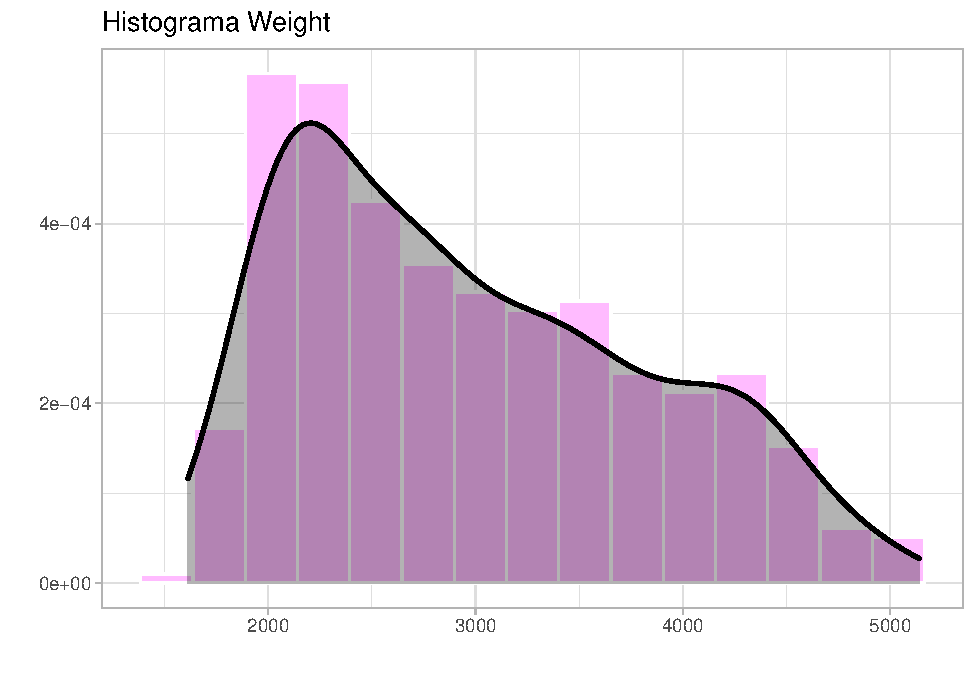
\includegraphics[width=.9\linewidth]{img/EDA_files/figure-latex/unnamed-chunk-7-3} \caption{}\end{figure}
\begin{figure}[H]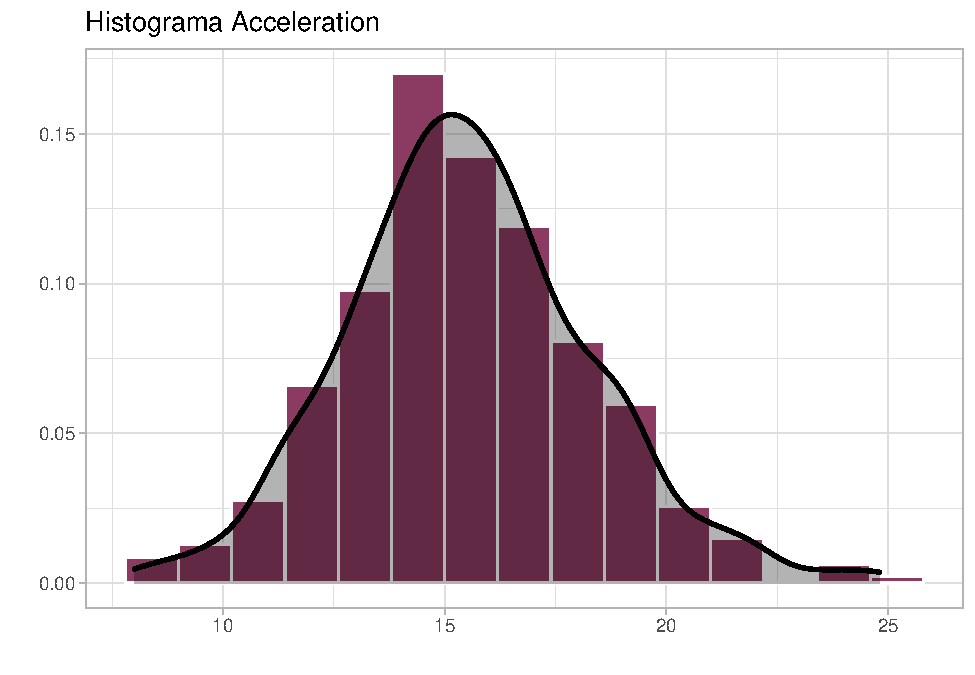
\includegraphics[width=.9\linewidth]{img/EDA_files/figure-latex/unnamed-chunk-7-4} \caption{}\end{figure}
\begin{figure}[H]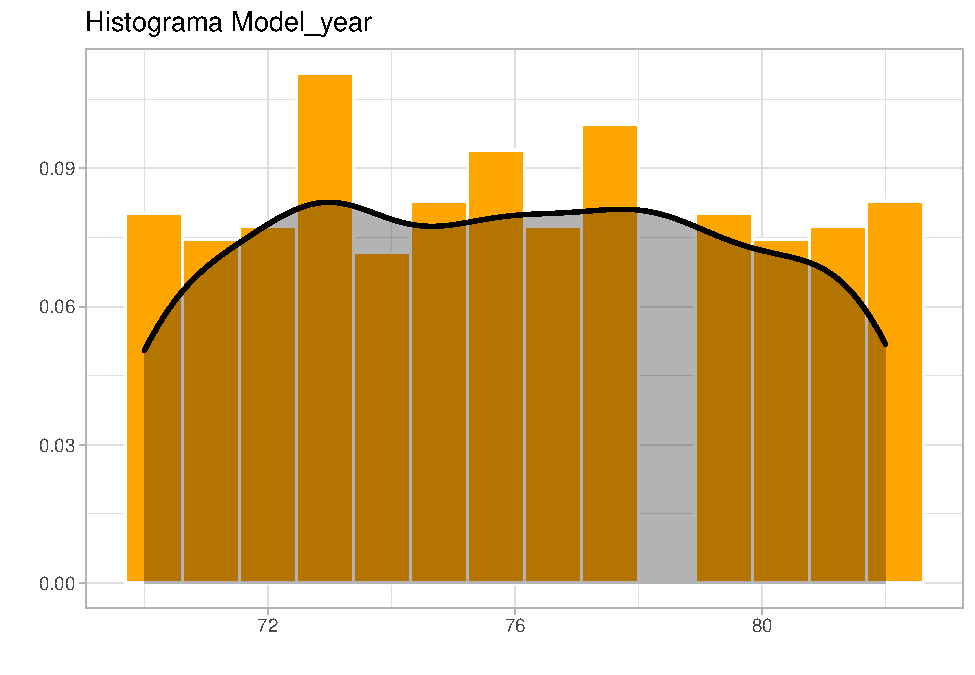
\includegraphics[width=.9\linewidth]{img/EDA_files/figure-latex/unnamed-chunk-7-5} \caption{}\end{figure}
\begin{figure}[H]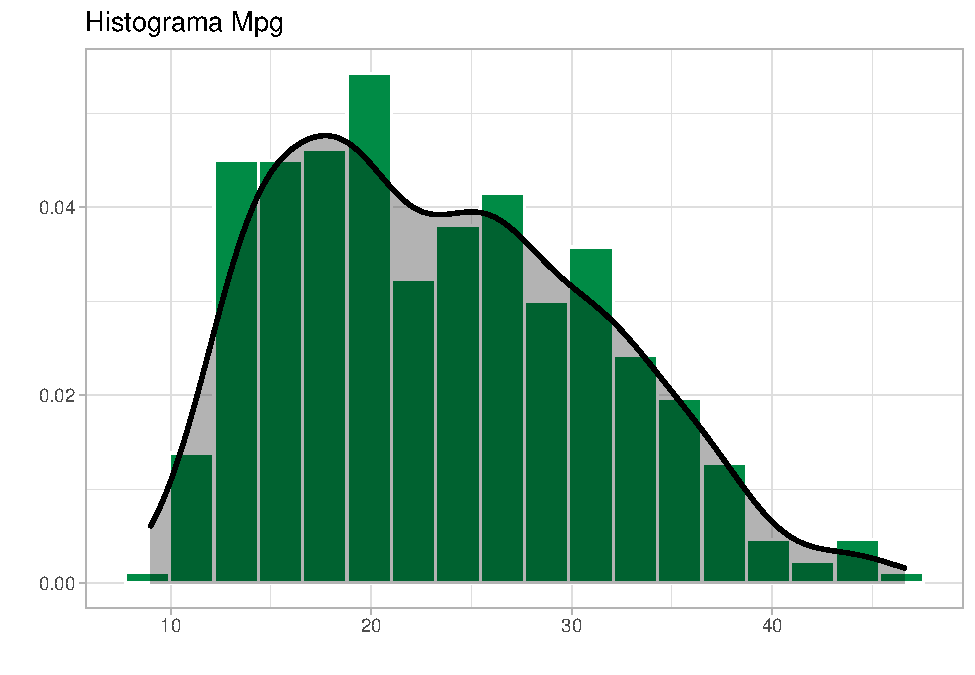
\includegraphics[width=.9\linewidth]{img/EDA_files/figure-latex/unnamed-chunk-7-6} \caption{}\end{figure}

\begin{figure}[H]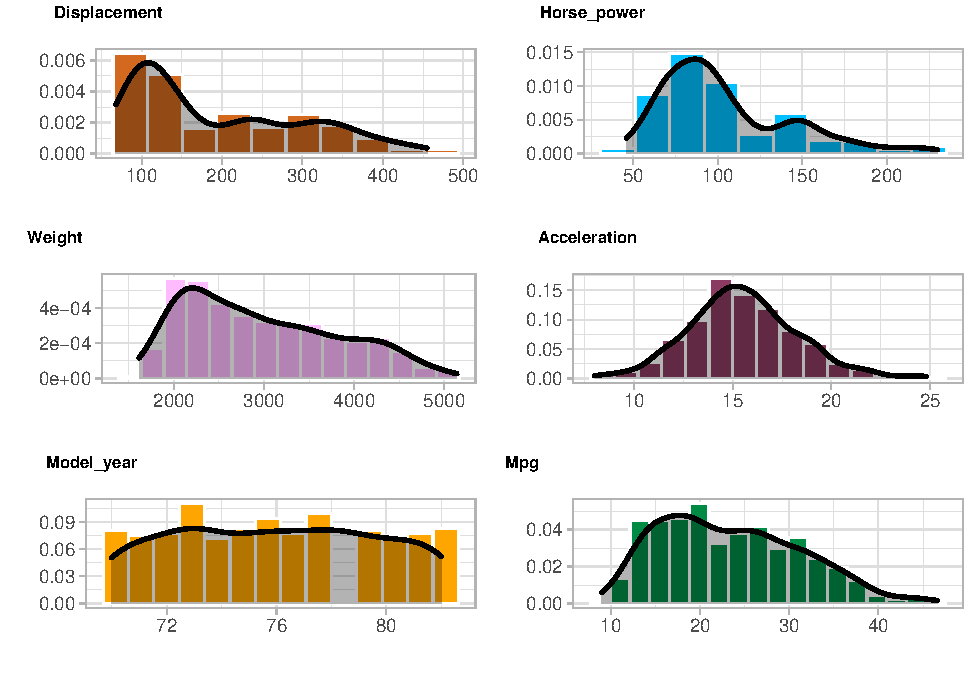
\includegraphics[width=.9\linewidth]{img/EDA_files/figure-latex/unnamed-chunk-7-7} \caption{}\end{figure}

Y boxplots sobre las distribuciones de los datos:
\begin{figure}[H]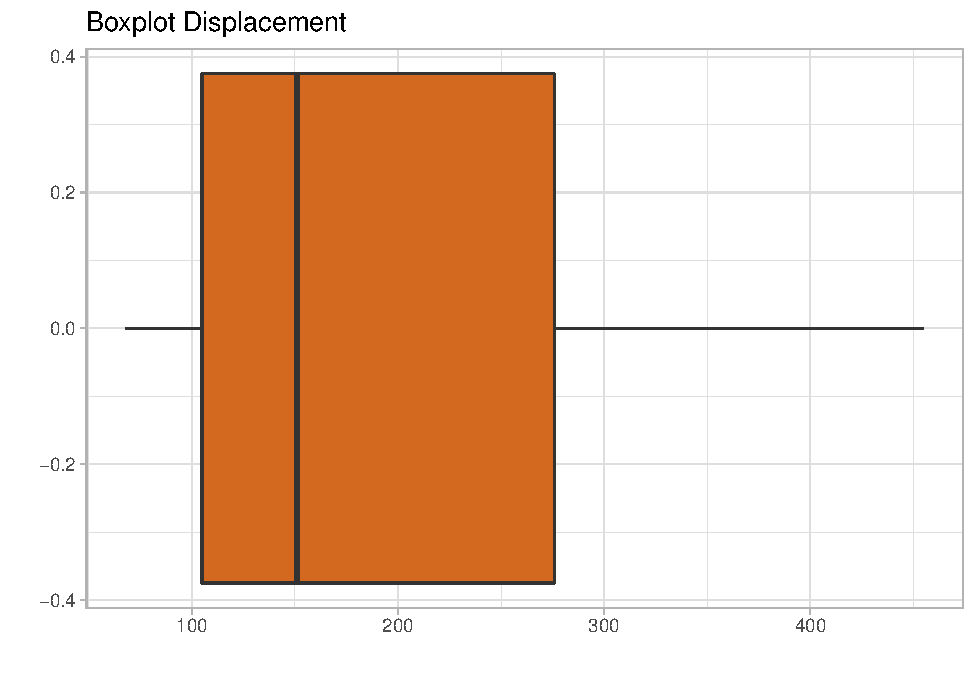
\includegraphics[width=.9\linewidth]{img/EDA_files/figure-latex/unnamed-chunk-8-1} \caption{}\end{figure}
\begin{figure}[H]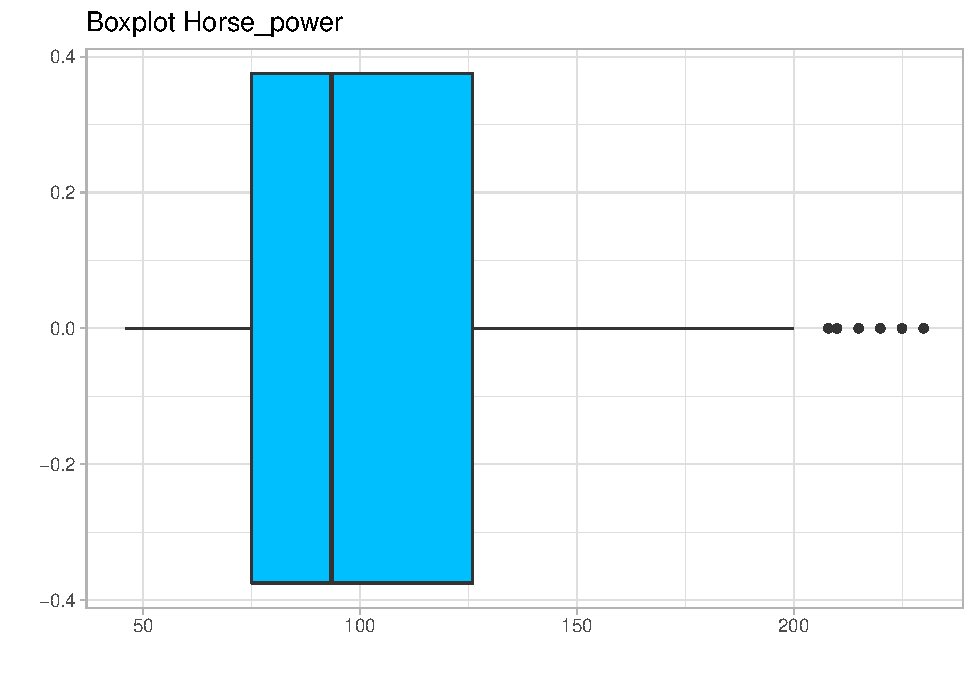
\includegraphics[width=.9\linewidth]{img/EDA_files/figure-latex/unnamed-chunk-8-2} \caption{}\end{figure}
\begin{figure}[H]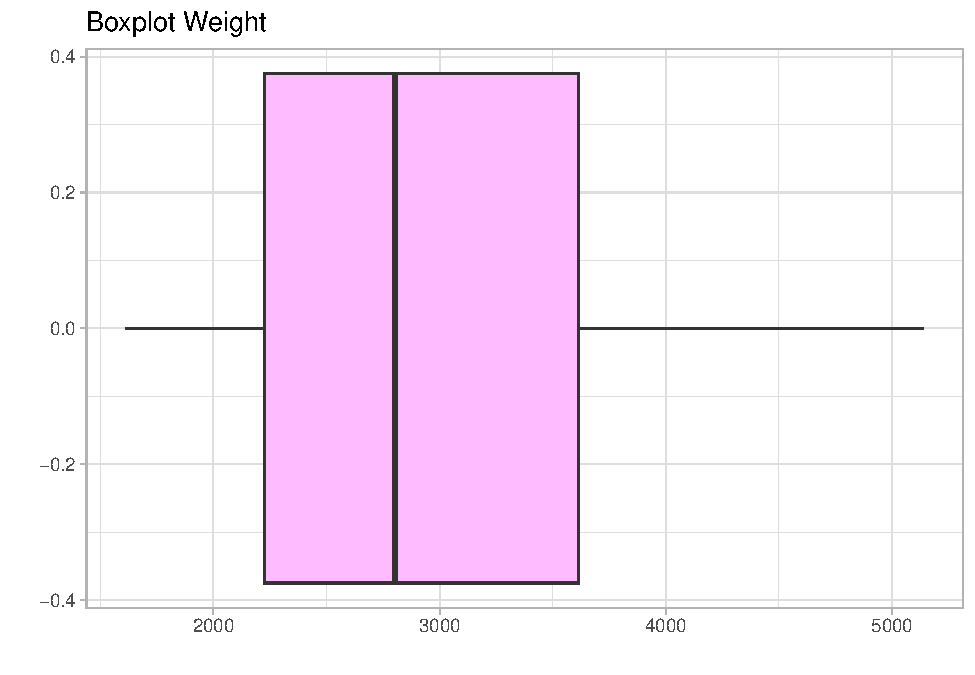
\includegraphics[width=.9\linewidth]{img/EDA_files/figure-latex/unnamed-chunk-8-3} \caption{}\end{figure}
\begin{figure}[H]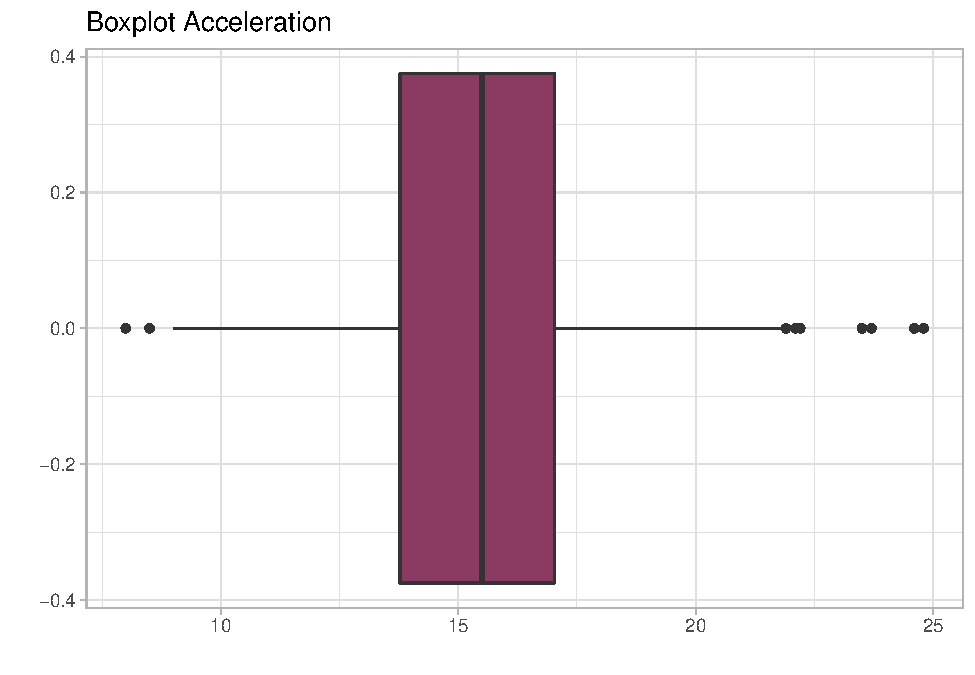
\includegraphics[width=.9\linewidth]{img/EDA_files/figure-latex/unnamed-chunk-8-4} \caption{}\end{figure}
\begin{figure}[H]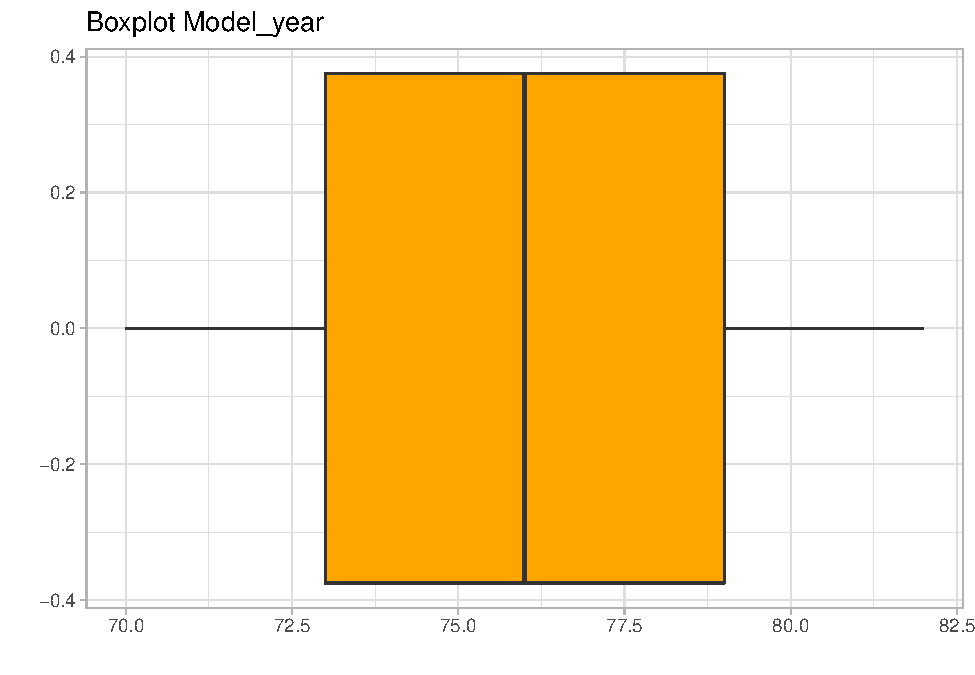
\includegraphics[width=.9\linewidth]{img/EDA_files/figure-latex/unnamed-chunk-8-5} \caption{}\end{figure}
\begin{figure}[H]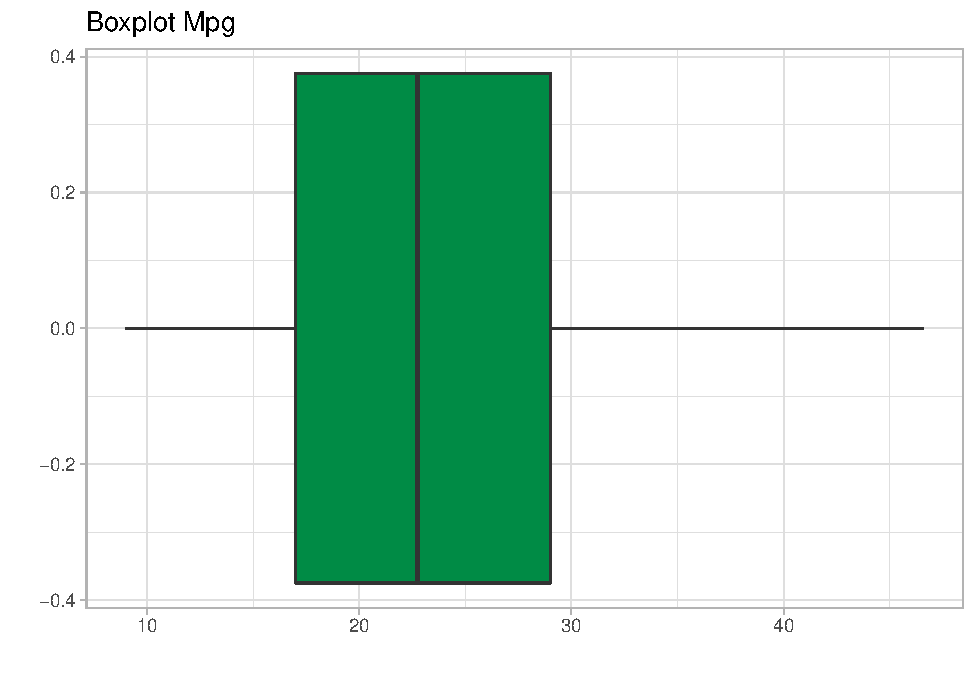
\includegraphics[width=.9\linewidth]{img/EDA_files/figure-latex/unnamed-chunk-8-6} \caption{}\end{figure}

\begin{figure}[H]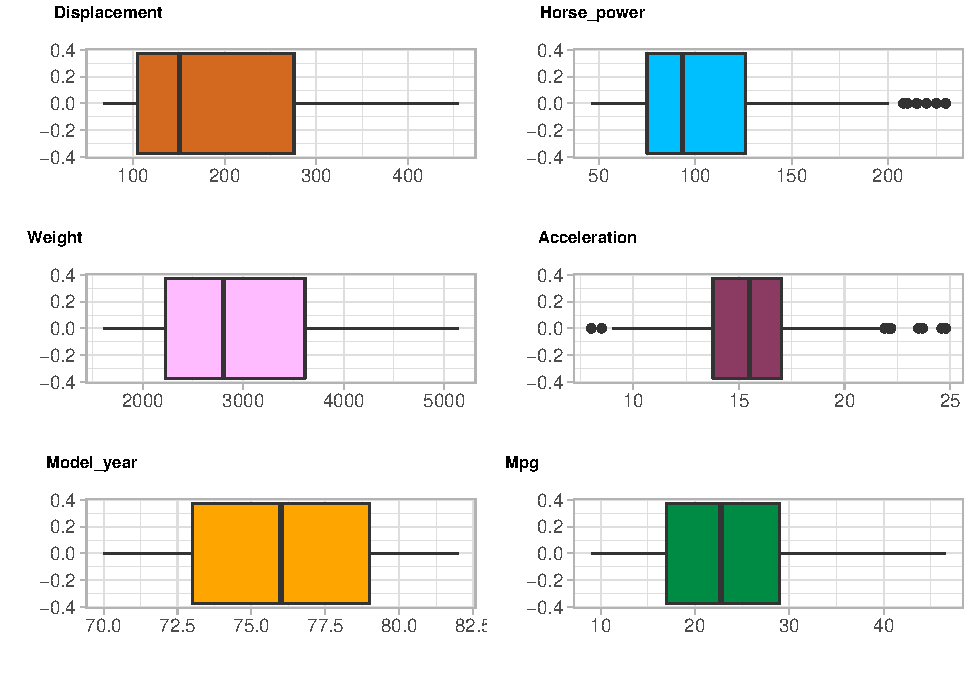
\includegraphics[width=.9\linewidth]{img/EDA_files/figure-latex/unnamed-chunk-8-7} \caption{}\end{figure}
\begin{figure}[H]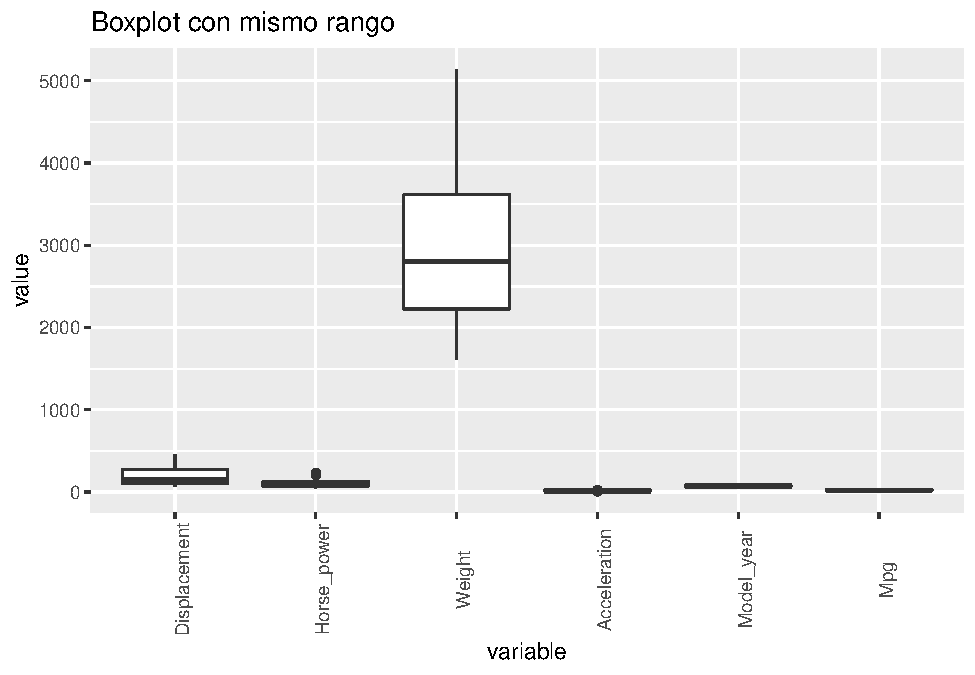
\includegraphics[width=.9\linewidth]{img/EDA_files/figure-latex/unnamed-chunk-9-1} \caption{}\end{figure}
\begin{figure}[H]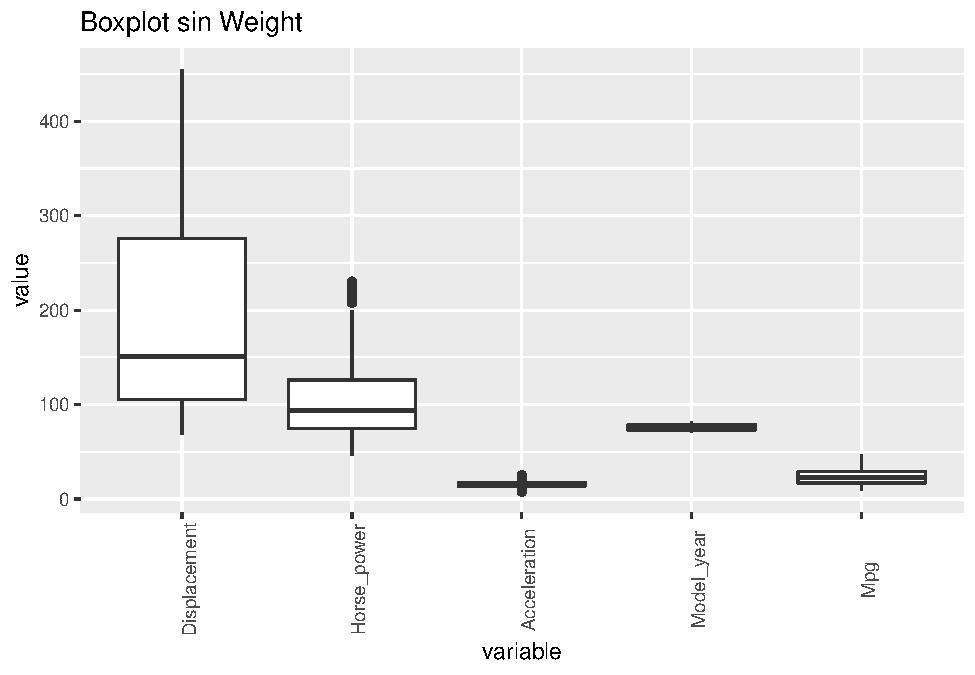
\includegraphics[width=.9\linewidth]{img/EDA_files/figure-latex/unnamed-chunk-9-2} \caption{}\end{figure}

Ya la descripción del problema nos lo decía, los rangos en los que se distribuyen los datos son muy diferentes dependiendo de la variable. Se pueden estandarizar los datos para solucionar este problema, aunque para regresión lineal no es necesario (sí lo es para KNN)
\vspace{\baselineskip}
Podemos comparar los rangos intercuartiles si estandarizamos antes el dataset

\begin{verbatim}
Displacement  Horse_power       Weight Acceleration   Model_year          Mpg 
    1.631723     1.324980     1.635856     1.178021     1.628781     1.537475 
\end{verbatim}

También podemos ver la distancia entre mínimos y máximos

\begin{verbatim}
Displacement  Horse_power       Weight Acceleration   Model_year          Mpg 
    3.698253     4.780318     4.152330     6.089463     3.257562     4.817420 
\end{verbatim}

\paragraph{Displacement}
La cilindrada vemos con una desviación grande y una gran concentración en los valores inferiores. Desviado a la izquierda, no parece seguir una distribución normal. Existe una alta concentración en torno al valor 125, muy por encima del recuento que alcanzan el resto de valores

\paragraph{Horse\_power}
Similar a Displacement pero cuenta con una mayor dispersión y algunos valores muya altos. A día de hoy los coches suelen rondar los 120 en turismos y los 200 en SUVs. Aquí contamos con predominancia en el rango aproximado {[}70, 125{]} con algunas instancias por encima de los 200.
Desviado a la izquierda, no parece seguir una distribución normal.


\paragraph{Weight}
Una distribución más achatada que las anteriores, también ladeada hacia la izquierda. Un rango mayor

\paragraph{Acceleration}
Valores altamentes concentrados pero en general con un rango alto. Su forma se asemeja a una distribución normal.


\paragraph{Model\_year}
Aunque no se vea bien en las gráficas, contamos con valores de todos los años, más o menos equitativamente

\begin{verbatim}
Años:   70 71 72 73 74 75 76 77 78 79 80 81 82 
Conteo: 29 27 28 40 26 30 34 28 36 29 27 28 30 
\end{verbatim}


\subsubsection{Análisis sobre las distribuciones}

Hemos comentado antes que no apreciamos semejanzas con una distribución normal en algunas de las variables, lo comprobamos con un test estadístico (Shapiro-Wilk test):
\vspace{\baselineskip}
\begin{tabular}{l|r|r|r}
\hline
vars & statistic & p\_value & sample\\
\hline
Displacement & 0.8818359 & 0.0000000 & 392\\
\hline
Horse\_power & 0.9040975 & 0.0000000 & 392\\
\hline
Weight & 0.9414661 & 0.0000000 & 392\\
\hline
Acceleration & 0.9918671 & 0.0305289 & 392\\
\hline
Model\_year & 0.9469666 & 0.0000000 & 392\\
\hline
Mpg & 0.9671696 & 0.0000001 & 392\\
\hline
\end{tabular}

\vspace{\baselineskip}

El test de Shapiro nos asegura con bastante certeza que ninguna variable sigue una distribución normal, aunque en menor grado en Acceleration (sigue siendo al 97\% de confianza).

Para los modelos de regresión que vamos a usar aún así la normalidad de los datos no es necesaria.
\vspace{\baselineskip}
Se muestra aquí como no hay que dejarse engañar por los gráficos, puesto que Acceleration parecía seguirla. El p-value de Acceleration está muy cerca del umbral (0.03 vs 0.05). Es bastante probable de que la parte central derecha de la distribución sea la causante de no asegurar la normalidad.

\vspace{\baselineskip}
Mostramos con gráficos Q-Q cómo se separan las distribuciones de su supuesta normal:

\begin{figure}[H]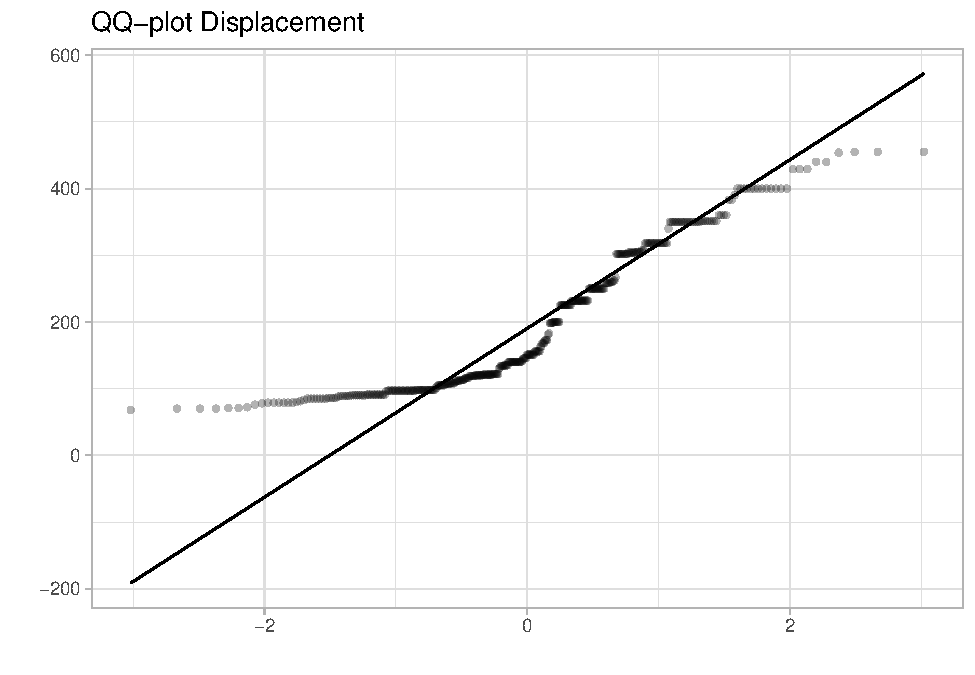
\includegraphics[width=.9\linewidth]{img/EDA_files/figure-latex/unnamed-chunk-14-1} \caption{}\end{figure}

\begin{figure}[H]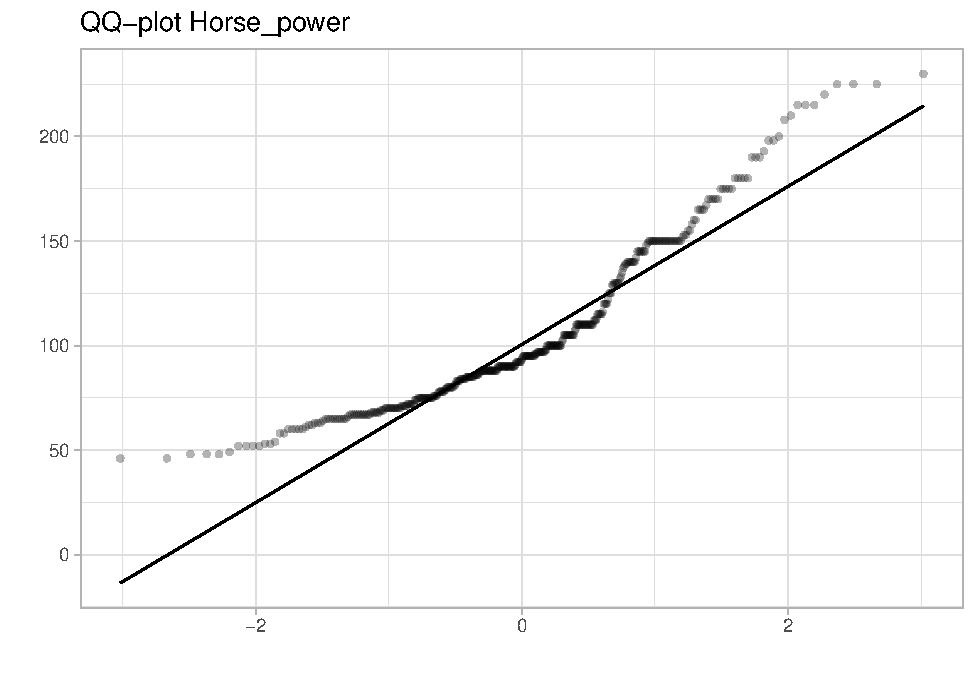
\includegraphics[width=.9\linewidth]{img/EDA_files/figure-latex/unnamed-chunk-14-2} \caption{}\end{figure}

\begin{figure}[H]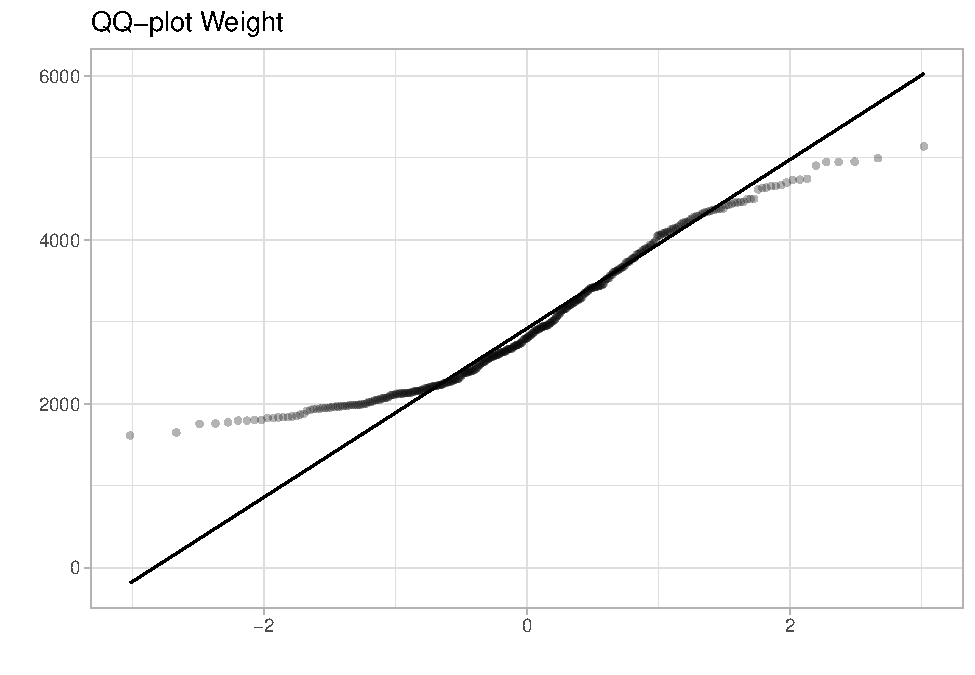
\includegraphics[width=.9\linewidth]{img/EDA_files/figure-latex/unnamed-chunk-14-3} \caption{}\end{figure}

\begin{figure}[H]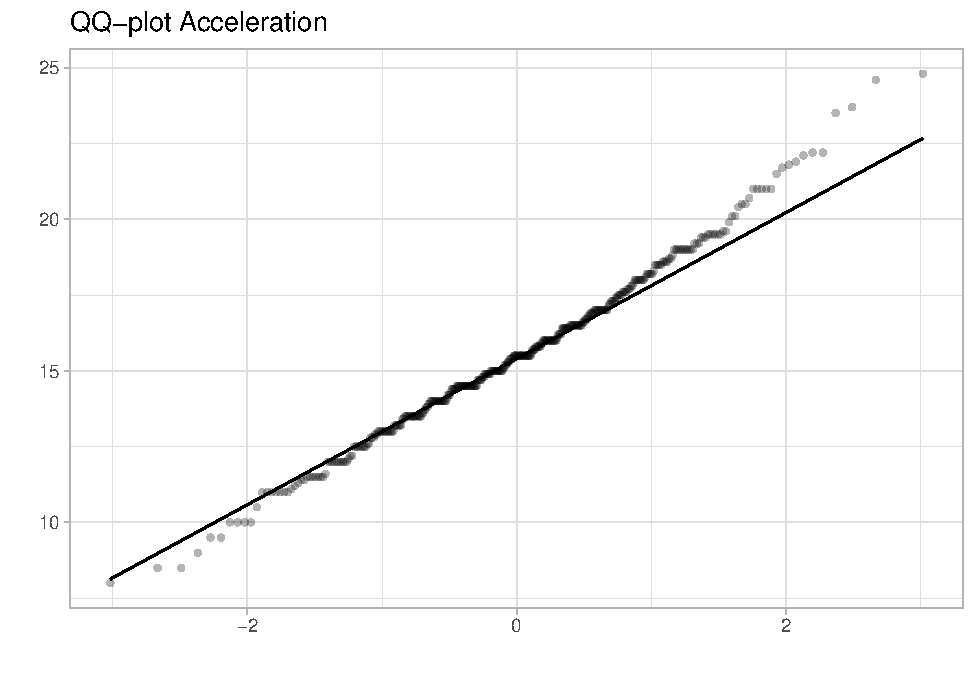
\includegraphics[width=.9\linewidth]{img/EDA_files/figure-latex/unnamed-chunk-14-4} \caption{}\end{figure}

\begin{figure}[H]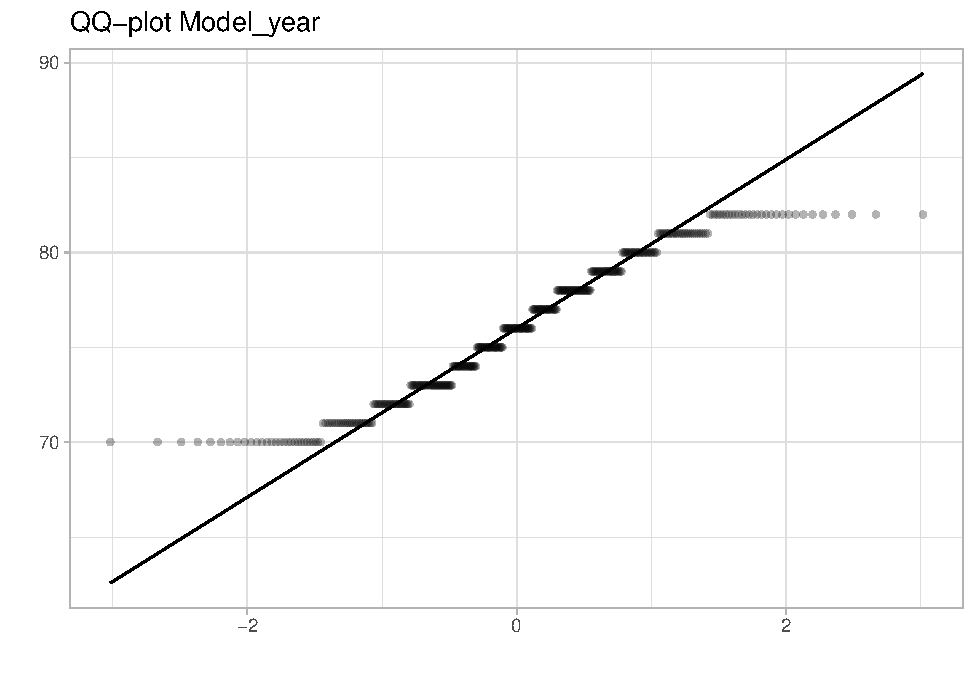
\includegraphics[width=.9\linewidth]{img/EDA_files/figure-latex/unnamed-chunk-14-5} \caption{}\end{figure}

\begin{figure}[H]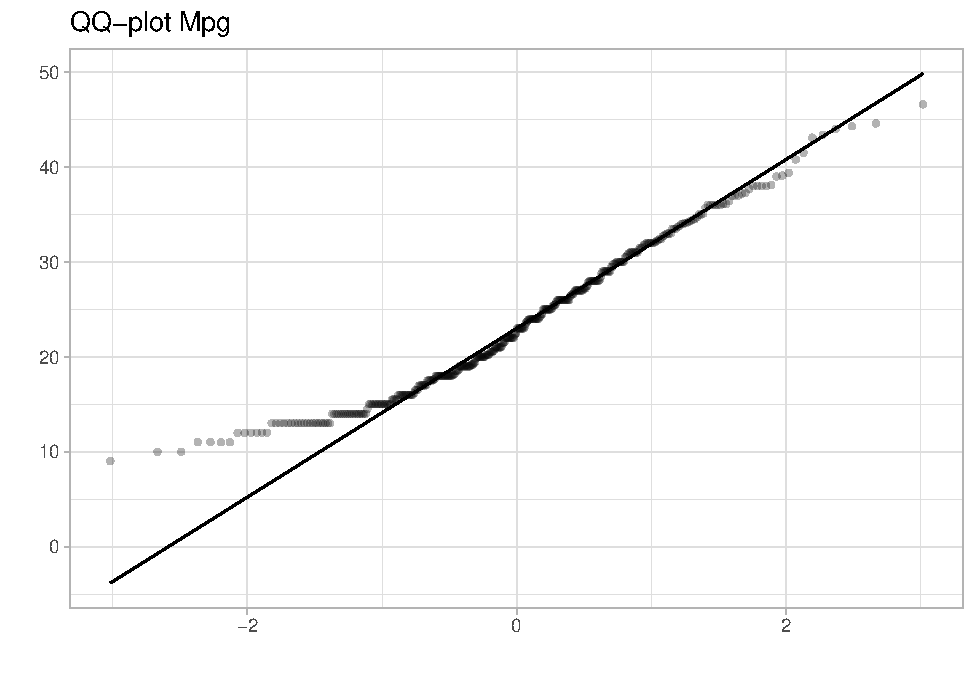
\includegraphics[width=.9\linewidth]{img/EDA_files/figure-latex/unnamed-chunk-14-6} \caption{}\end{figure}

\begin{figure}[H]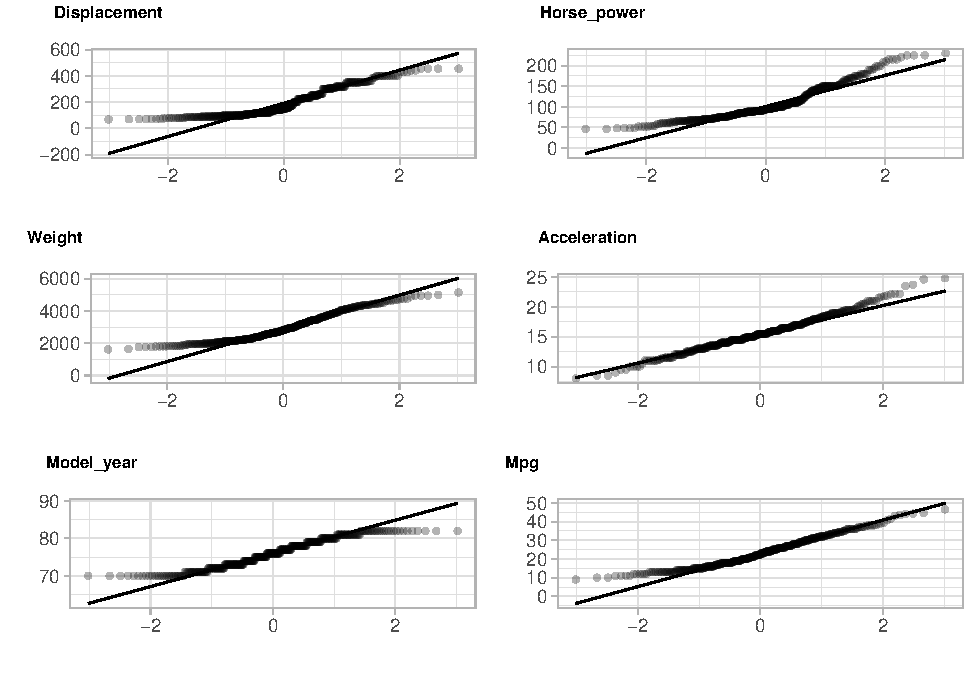
\includegraphics[width=.9\linewidth]{img/EDA_files/figure-latex/unnamed-chunk-14-7} \caption{}\end{figure}

Estos gráficos Q-Q nos muestran más claramente que las variables no siguen distribuciones normales. La distribución de Acceleration es la que más se asemeja y eso lo vemos en el estadístico de Shapiro, pero en la cola superior existe una diferencia significativa que hace que el test rechace.

\paragraph{Skewness}
Las variables con skewness que tenemos son:

\begin{verbatim}
"Displacement" "Horse_power"  "Weight"      
\end{verbatim}

Concretamente, sus valores son:

\begin{verbatim}
Displacement: [1] 0.6989813
Horse_power: [1] 1.083161
Weight: [1] 0.5175953

Adicionalmente, se muestra:
Mpg: [1] 0.4553414
\end{verbatim}

Sobre la skewness, tal y como se había visto en las gráficas, algunas de las variables la tienen, en los 3 casos positivas (hacia la izquierda).

Los plots nos han dado idea de que Mpg tiene cierta skewness, pero cae por debajo del umbral de 0.5.

\subsubsection{Transformaciones}
En general no consideramos ninguna transformación necesaria para el dataset con el que contamos.
No vemos necesario crear variables nuevas a partir de las vistas, puesto que por el conocimiento que tenemos del problema parece que las variables son coherentes.

Las transformaciones necesarias para pasar a una distribución normal dependen de la variable en cuestión. Primero deberíamos averiguar que tipo de distribución siguen.
Aunque, tal y como se ha comentado anteriormente, los métodos utilizados para regresión (regresión lineal y KNN) no asumen ninguna forma para la distribución de los datos, por lo que no es necesario aplicar nada.

Adicionalmente, aunque para regresión lineal no es absolutamente necesario, podemos estandarizar los datos a media 0 y dev 1, facilitando un poco los cálculos. La inferencia estadística de la regresión no variaría aplicando esta transformación, pero deberíamos tener cuidado a la hora de interpretar los resultados de la regresión para no confundirnos.

\subsubsection{Outliers}

Como hemos visto anteriormente en los boxplots, las únicas variables con valores muy alejados del centro de la distribución son Acceleration y Horse\_power.

Por el significado del problema, probablemente estos posibles outliers correspondan a coches de alta gama o potentes en la época. Esto tampoco lo podemos asegurar puesto que contamos con pocas características, pero se considera un razonamiento coherente. Además, puesto que los valores caen dentro de los rangos posibles para coches de la época, podemos descartar que sean errores de medida.

Deberíamos decidir si mantener o no estas instancias. Como en nuestro caso se nos ha pedido predecir el consumo Mpg, sin darnos consideraciones sobre los tipos/gamas de coches a los que se enfoca, proseguimos dejándo estas filas.

\subsubsection{Análisis de correlación}

Tenemos que tener en cuenta que las variables no siguen distribuciones normales. Aunque el coeficiente de Pearson no asume normalidad (si asume varianza y covarianza finitas), podemos además usar el coeficiente de Kendall para los cálculos. Independientemente del método usado vamos a obtener las mismas correlaciones en este dataset, solo varía el valor de fuerza con la que se dan.

\vspace{\baselineskip}

Para regresión la correlación en los datos no es preocupante. Al contrario, podría haber información (poca, pero alguna cantidad) que se aporte y nos ayude en el problema. En el peor de los casos, la propia metodología de selección de variables en el modelo multivariable nos ayudará a descartar aquellas variables que no sean necesarias como regresor.

\begin{figure}[H]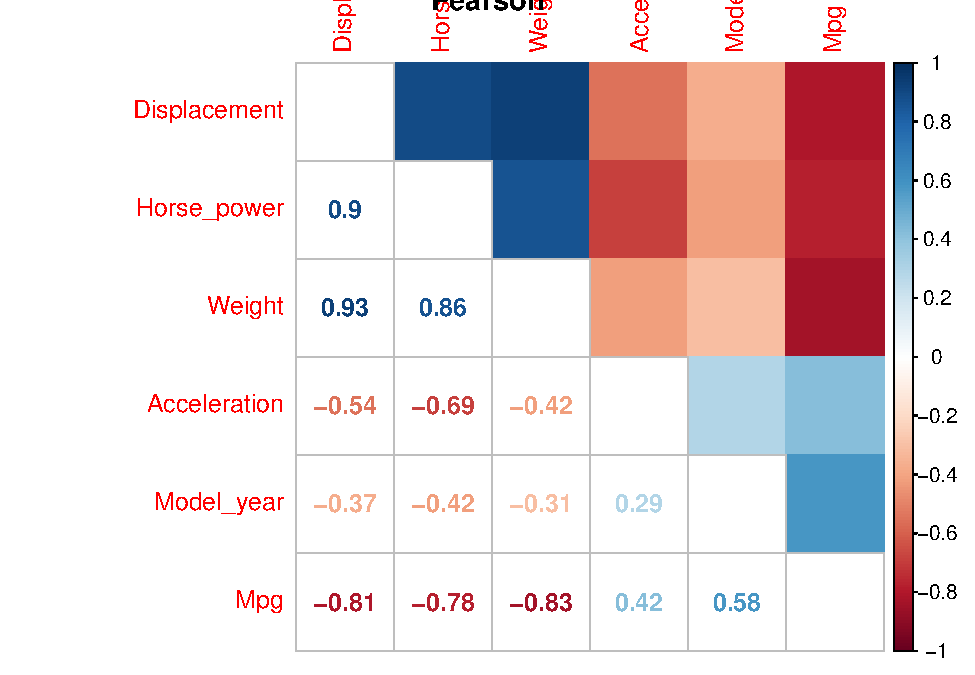
\includegraphics[width=.9\linewidth]{img/EDA_files/figure-latex/unnamed-chunk-19-1} \caption{}\end{figure}
\begin{figure}[H]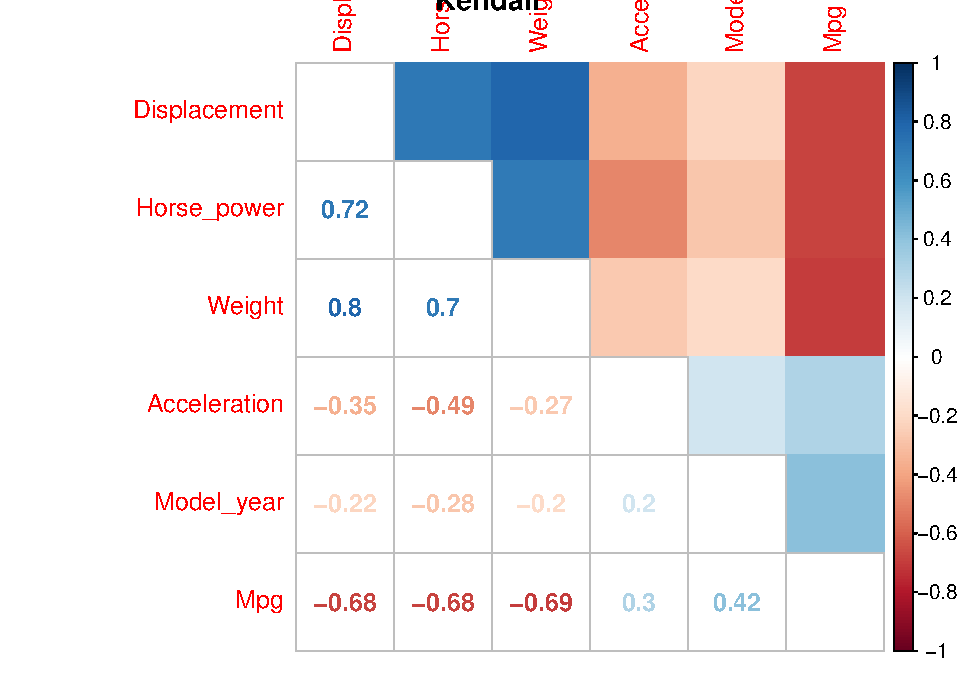
\includegraphics[width=.9\linewidth]{img/EDA_files/figure-latex/unnamed-chunk-19-2} \caption{}\end{figure}

Estas gráficas nos dicen que existe una alta correlación en el dataset, generalmente entre todas las variables (a excepción de Model\_year), pero extremadamente fuerte en las parejas:

\begin{enumerate}
    \def\labelenumi{\arabic{enumi}.}
    \item   Horse\_power \& Displacement
    \item   Weight \& Displacement
    \item   Weight \& Horse\_power
    \item   Acceleration \& Horse\_power
    \item   Mpg \& Horse\_power
    \item   Mpg \& Displacement
    \item   Mpg \& Weight
\end{enumerate}

\begin{figure}[H]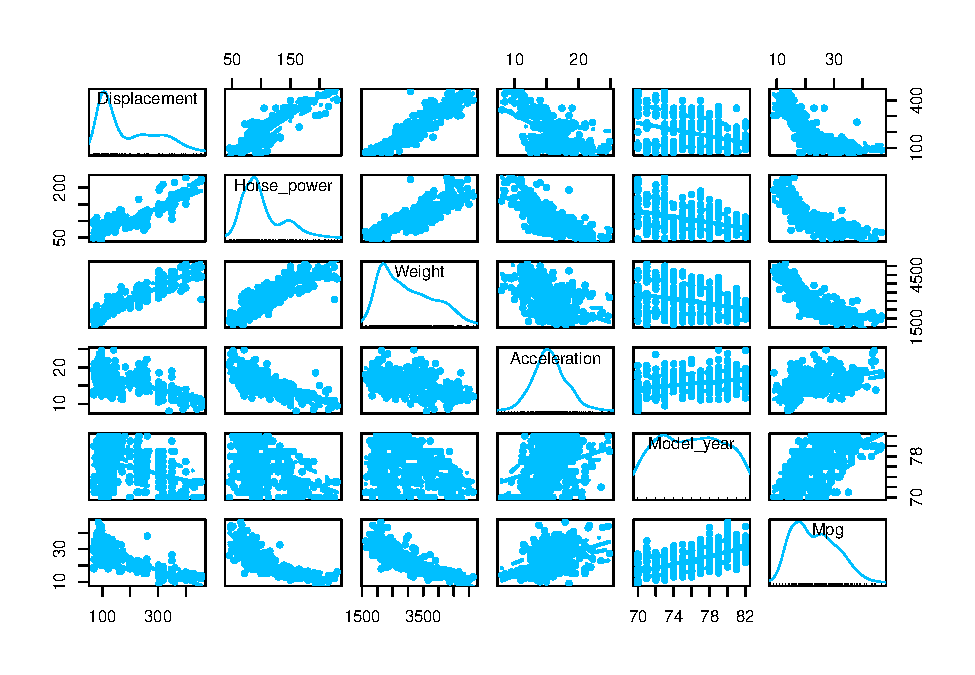
\includegraphics[width=.9\linewidth]{img/EDA_files/figure-latex/unnamed-chunk-20-1} \caption{}\end{figure}

El scatterplot anterior nos muestra mejor la forma de estas correlaciones. Vemos que en todos los casos en los que se da una correlación positiva existe una tendencia lineal entre los datos de ambas variables, y en las negativas una tendencia logarítmica.

\vspace{\baselineskip}

Vamos a mostrar algunas parejas con correlación positiva:

\begin{figure}[H]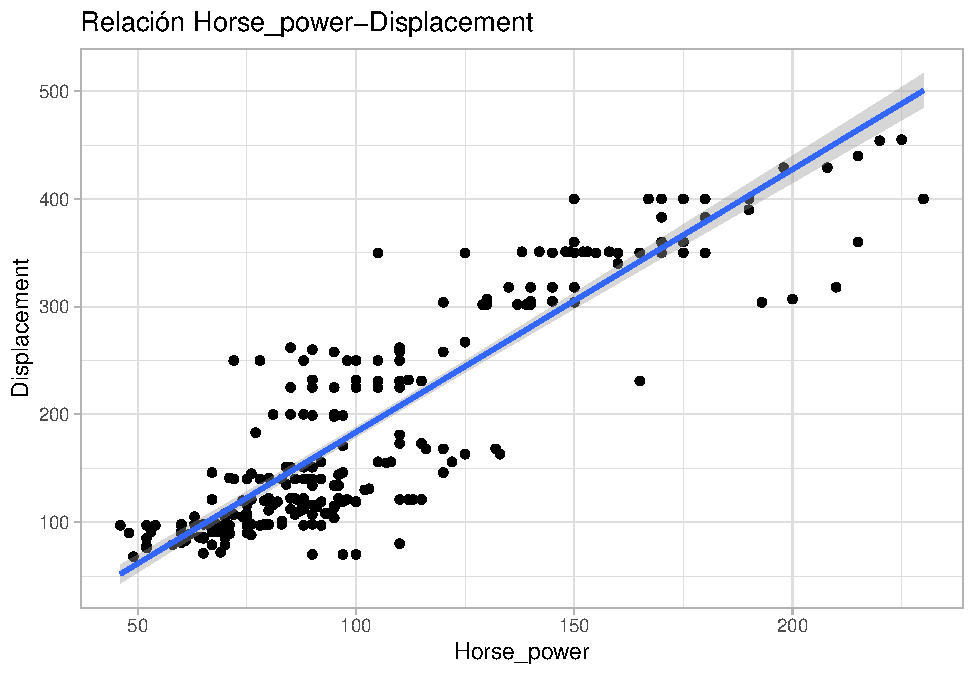
\includegraphics[width=.9\linewidth]{img/EDA_files/figure-latex/unnamed-chunk-21-1} \caption{}\end{figure}
\begin{figure}[H]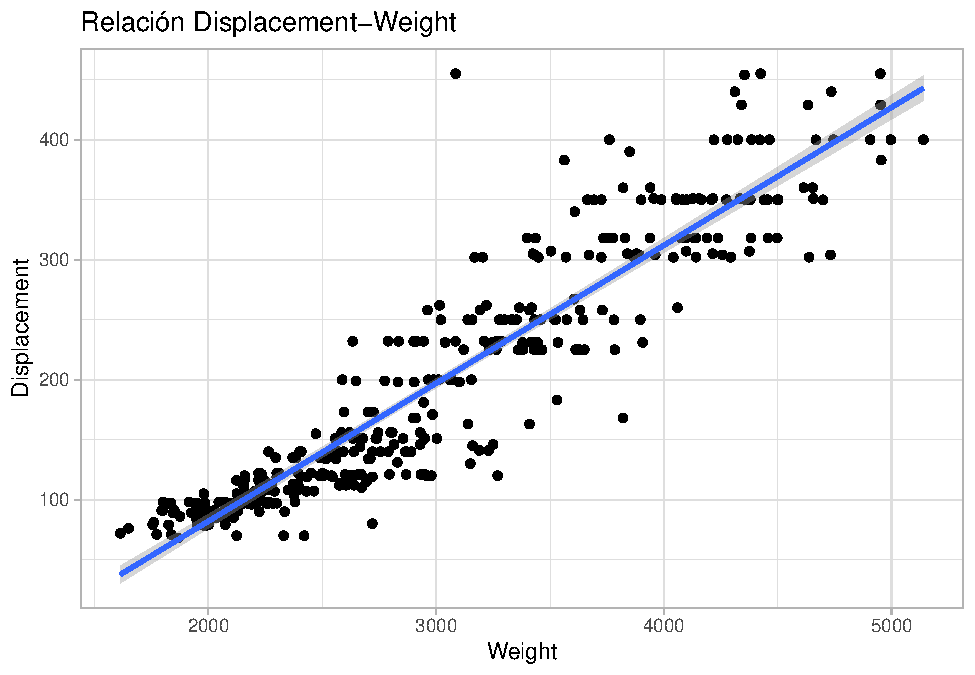
\includegraphics[width=.9\linewidth]{img/EDA_files/figure-latex/unnamed-chunk-21-2} \caption{}\end{figure}

Y otras con correlación negativa:

\begin{figure}[H]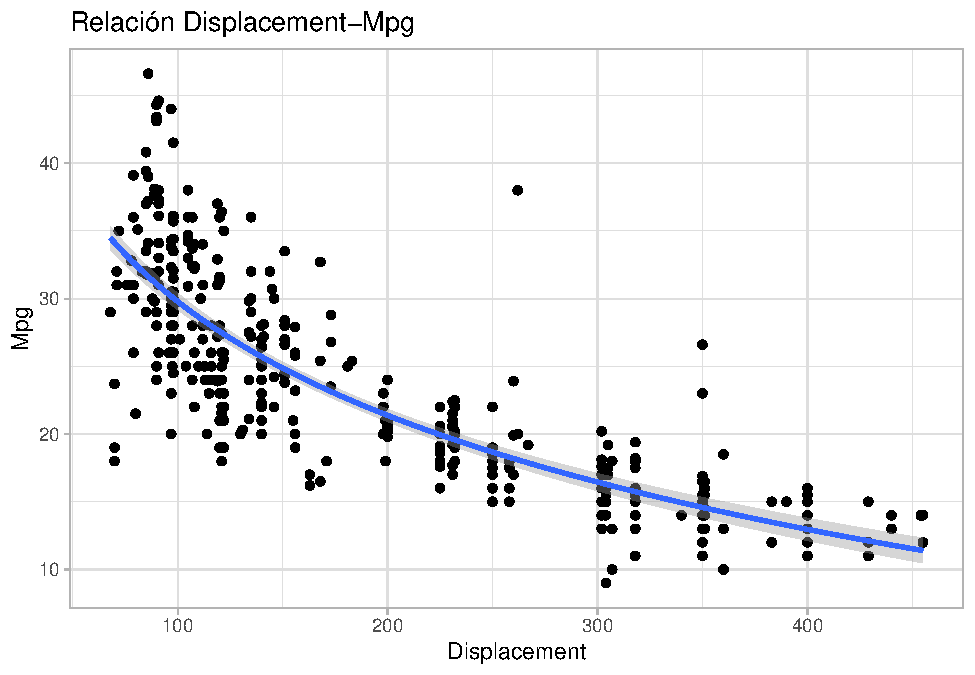
\includegraphics[width=.9\linewidth]{img/EDA_files/figure-latex/unnamed-chunk-22-1} \caption{}\end{figure}
\begin{figure}[H]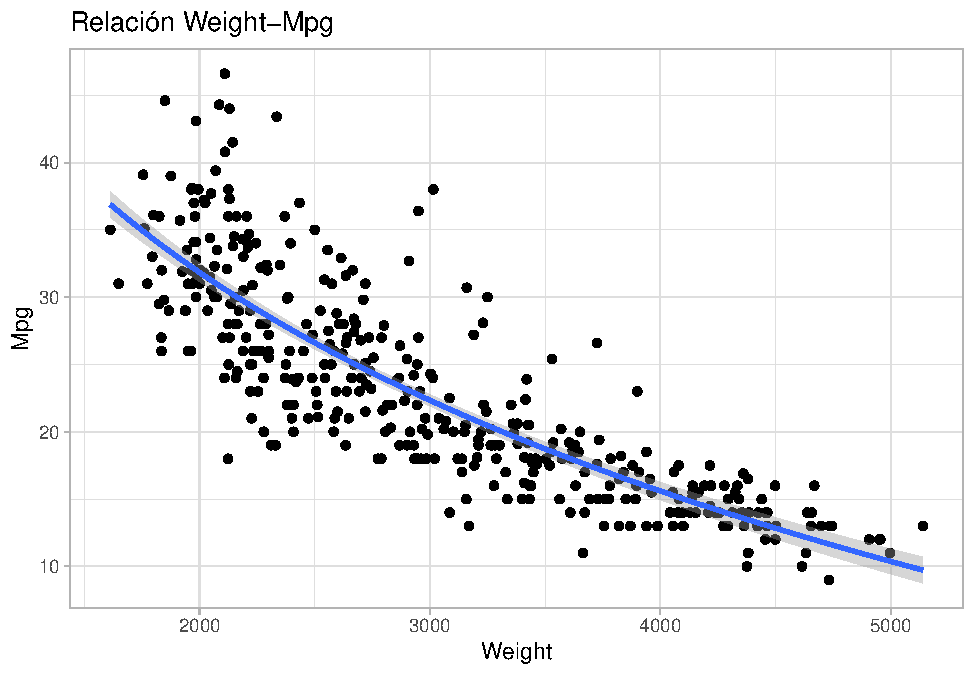
\includegraphics[width=.9\linewidth]{img/EDA_files/figure-latex/unnamed-chunk-22-2} \caption{}\end{figure}

También podemos visualizar los regresores respecto a la salida:

\begin{figure}[H]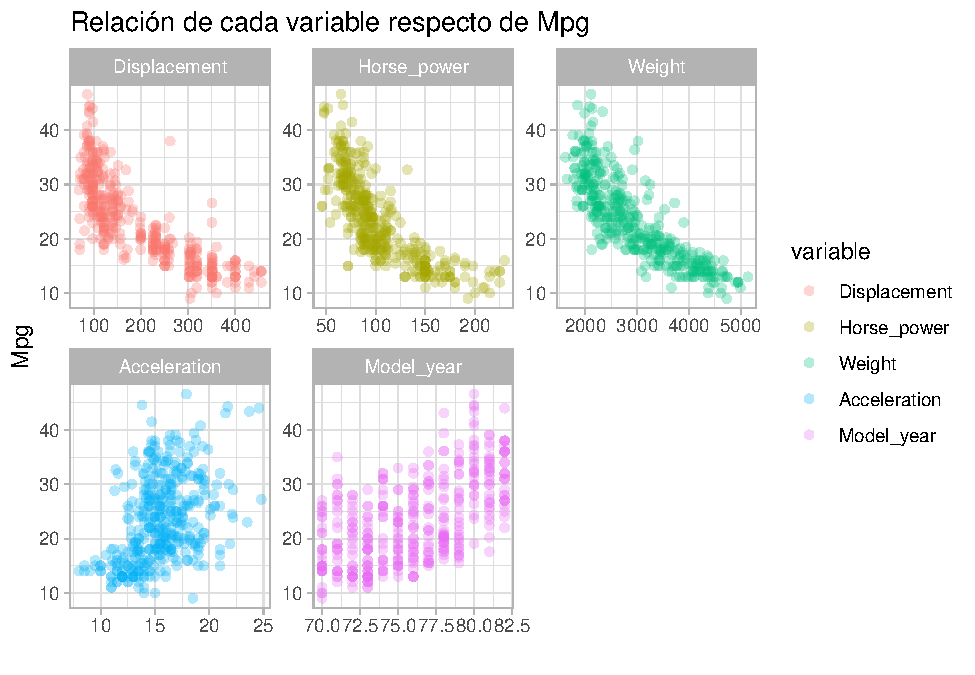
\includegraphics[width=.9\linewidth]{img/EDA_files/figure-latex/unnamed-chunk-23-1} \caption{}\end{figure}

Como habíamos visto, existe alta correlación entre Displacement, Horse\_power, Weight respecto de Mpg.

\vspace{\baselineskip}

Haciendo referencia a la hipótesis H.9, Horse\_power podría depender de Displacement y Weight. Parece bastante probable que la potencia de un motor dependa de la cilindrada y el peso que tenga.

\begin{figure}[H]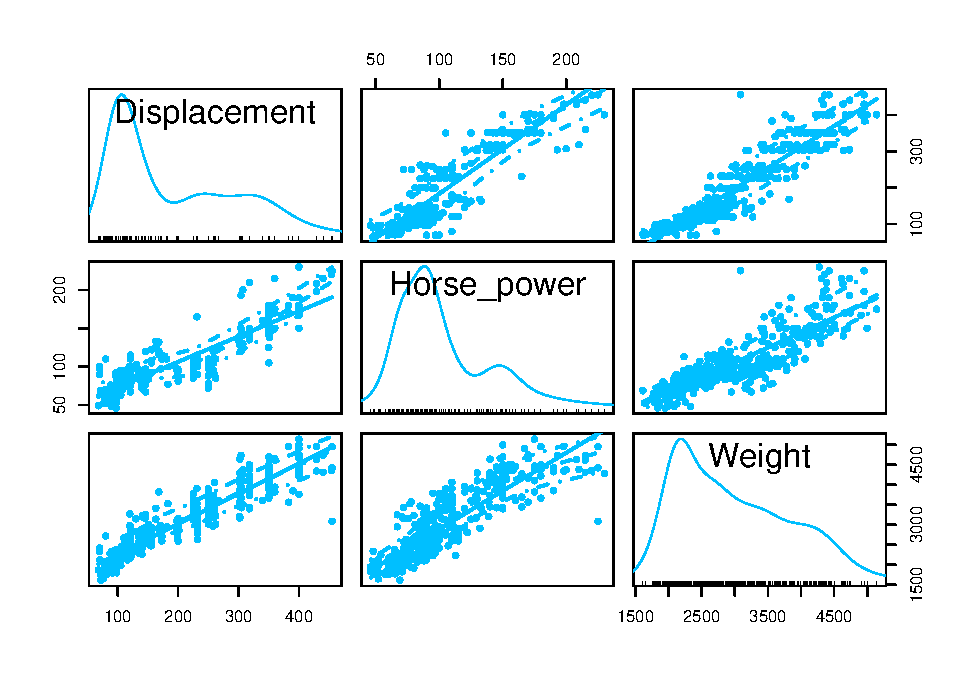
\includegraphics[width=.9\linewidth]{img/EDA_files/figure-latex/unnamed-chunk-24-1} \caption{}\end{figure}

% !!!!!!!!!!!!!!!!!!!!!!!!!!!!!!!!!!!!!!!!!!!!!!!!!!!!!!!!

Podemos apreciar como la función de densidad de Horse\_power parece una (``MEDIANIZACIÓN'') de las otras dos.

% !!!!!!!!!!!!!!!!!!!!!!!!!!!!!!!!!!!!!!!!!!!!!!!!!!!!!!!!

Vamos a intentar comprobarlo

\begin{figure}[H]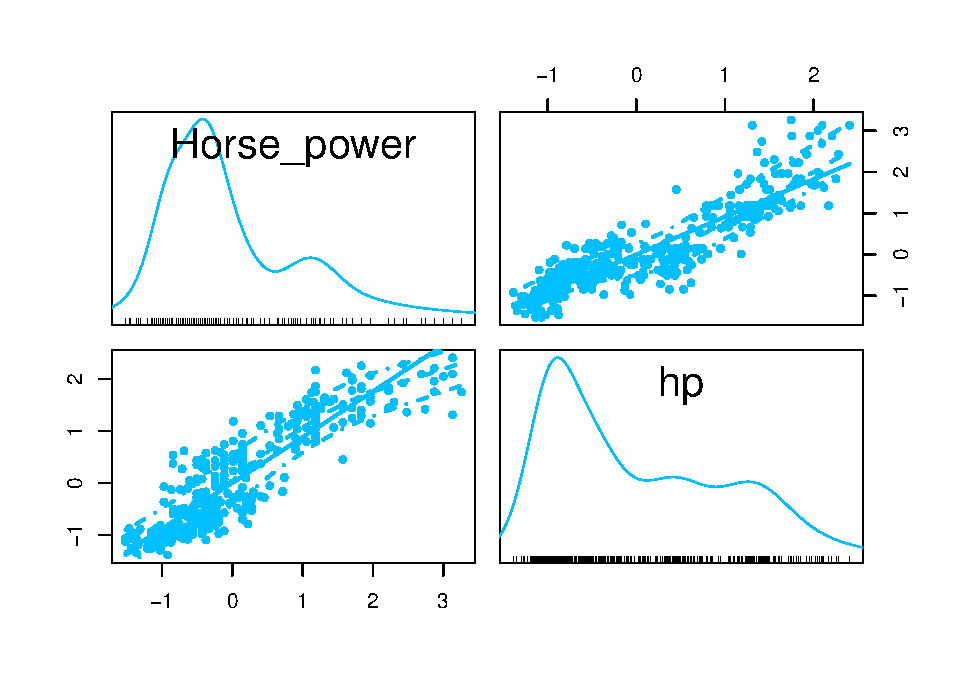
\includegraphics[width=.9\linewidth]{img/EDA_files/figure-latex/unnamed-chunk-25-1} \caption{}\end{figure}

Viendo que no son tan similares como creíamos, buscamos diferentes fórmulas para el cálculo de los caballos de vapor, y vemos que las fórmulas son un poco más complejas y no tenemos exactamente los datos necesarios para utilizarlas (no se descarta que no se puedan deducir, pero no sería un cálculo evidente)

(poner fórmulas
\url{https://www.ajdesigner.com/phphorsepower/horsepower_equation_trap_speed_method_increase_horsepower.php\#}:\textasciitilde:text=Solving\%20for\%20the\%20change\%20in,the\%20vehicle\%2C\%20driver\%20and\%20passenger.)

\subsubsection{Tratamiento de variables}

Para este dataset, al ser casi todas las variables numéricas continuas, existen pocos tratamientos que aplicar.

No tenemos variables categóricas que transformar.

Para añadir interpretabilidad, podríamos agrupar la variable Weight en intervalos, pero puesto que vamos a aplicar regresión sería más conveniente realizarlo con los resultados finales.

\subsubsection{Ordenaciones}

Volvemos a mostrar la cabecera de los datos:
\vspace{\baselineskip}

\begin{tabular}{r|r|r|r|r|r}
\hline
Displacement & Horse\_power & Weight & Acceleration & Model\_year & Mpg\\
\hline
91 & 70 & 1955 & 20.5 & 71 & 26.0\\
\hline
232 & 100 & 2789 & 15.0 & 73 & 18.0\\
\hline
350 & 145 & 4055 & 12.0 & 76 & 13.0\\
\hline
318 & 140 & 4080 & 13.7 & 78 & 17.5\\
\hline
113 & 95 & 2372 & 15.0 & 70 & 24.0\\
\hline
97 & 60 & 1834 & 19.0 & 71 & 27.0\\
\hline
\end{tabular}

En este caso no es necesario aplicar ninguna reorganización. Cada variable ocupa su propia columna y contiene un único tipo de información, con unidades de observación diferentes. No existe ninguna relación entre variables sobre la información que codifican (en el sentido de que podrían agruparse).

\subsubsection{Resolución de hipótesis}

Nos habíamos planteado las siguientes hipótesis

\begin{itemize}
\item \textbf{H.1}: Horse\_power puede influir en Mpg: A más potencia, más consumo.
\end{itemize}

\begin{figure}[H]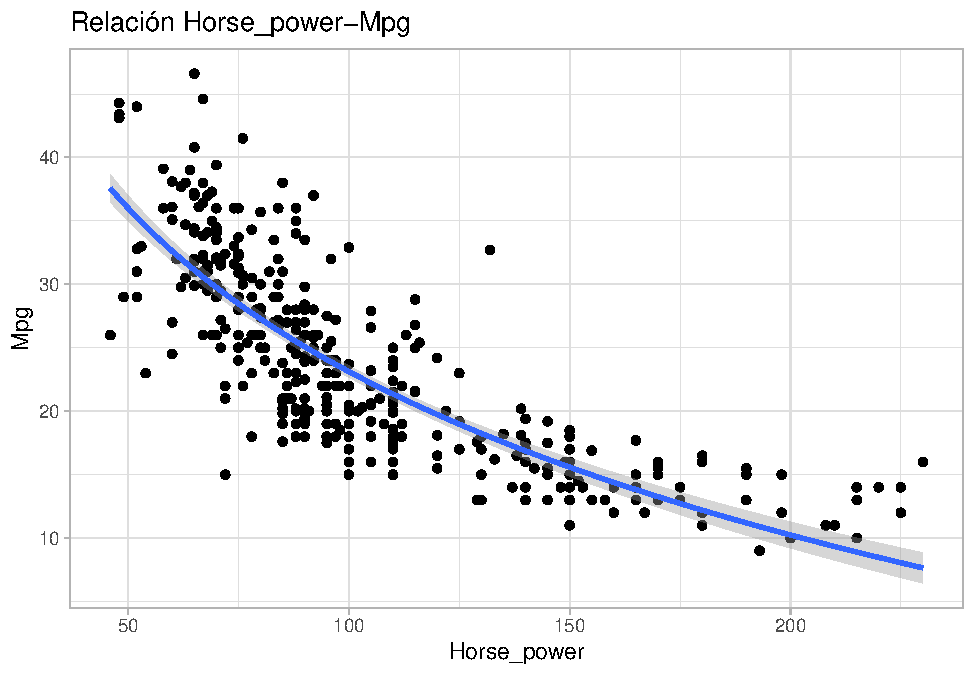
\includegraphics[width=.9\linewidth]{img/EDA_files/figure-latex/unnamed-chunk-27-1} \caption{}\end{figure}

Con el plot y los resultados de la matriz de correlación queda claro que existe una correlación negativa entre estas dos variables. Por tanto, podemos considerar Horse\_power como un buen candidato para la regresión

\begin{itemize}
\item \textbf{H.2}: Weight debe influir en Mpg: Un coche más pesado debería consumir más idem. a la hipótesis anterior, lo hemos visto anteriormente en la figura X
\item \textbf{H.3}: Debería haber correlación entre displacement (cilindrada) con horse y acceleration La hemos referenciado anteriormente
\item \textbf{H.4}: Horse y acceleration podrían estar relacionadas
\end{itemize}

\begin{figure}[H]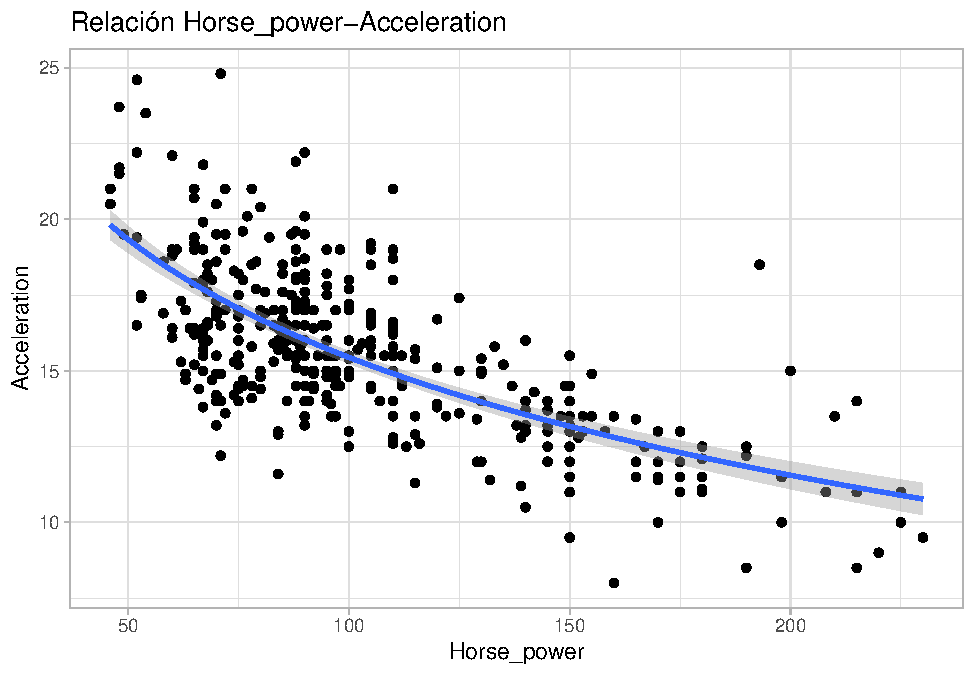
\includegraphics[width=.9\linewidth]{img/EDA_files/figure-latex/unnamed-chunk-28-1} \caption{}\end{figure}

idem. se aprecia una correlación logarítmica entre las dos variables. Similarmente a lo ocurrido con la hipótesis anterior, esto puede ser un problema para nuestro problema de regresión.

\begin{itemize}
\item \textbf{H.5}: Viendo que contamos con un rango pequeño de años, no debería haber un cambio significativo de prestaciones entre años.
\end{itemize}

\begin{figure}[H]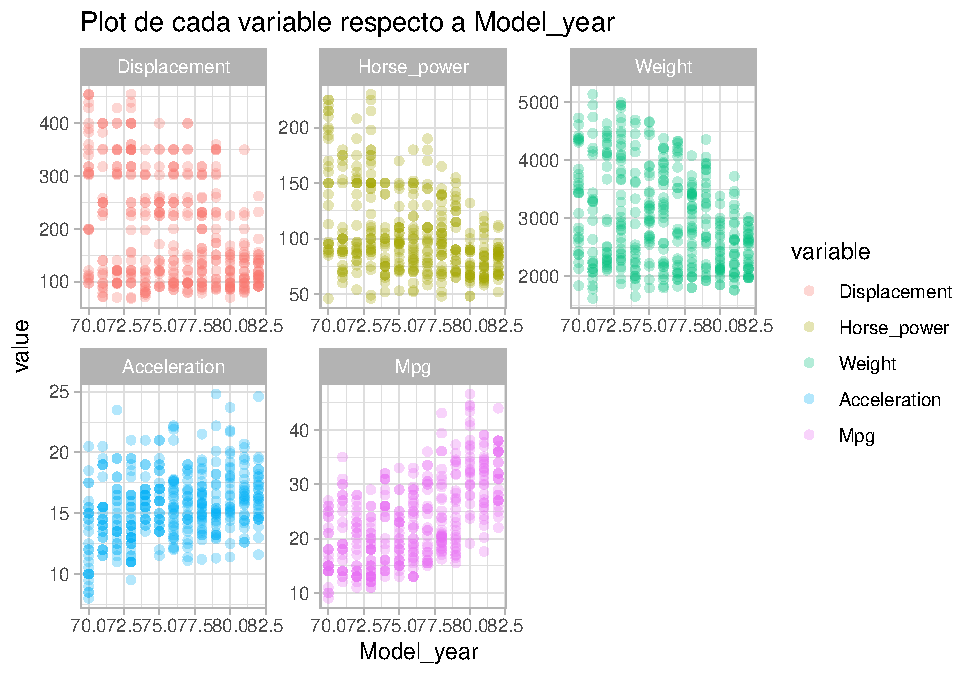
\includegraphics[width=.9\linewidth]{img/EDA_files/figure-latex/unnamed-chunk-29-1} \caption{}\end{figure}

Existe una alta dispersión de los datos en cada una de las variables, pero aún así se aprecia tendencias en las variables. Acceleartion y Mpg tienden a aumentar, y Displacement, Horse\_power y Weight tienden a disminuir. También vemos que la dispersión en las prestaciones de los coches disminuyen ligeramente.

Podemos creer en principio que puede deberse a un decremento del número de instancias con el paso de los años, pero recordamos que en general los datos están repartidos equitativamente

\begin{verbatim}
Años:   70 71 72 73 74 75 76 77 78 79 80 81 82 
Conteo: 29 27 28 40 26 30 34 28 36 29 27 28 30 
\end{verbatim}

Podemos ver cómo varían los rangos para cada año

\begin{verbatim}
Year: 70  Displacement Horse_power Weight Acceleration Model_year Mpg
1           97          46   1835          8.0         70   9
2          455         225   4732         20.5         70  27
Year: 71  Displacement Horse_power Weight Acceleration Model_year Mpg
1           71          60   1613         11.5         71  12
2          400         180   5140         20.5         71  35
Year: 72  Displacement Horse_power Weight Acceleration Model_year Mpg
1           70          54   2100         11.0         72  11
2          429         208   4633         23.5         72  28
Year: 73  Displacement Horse_power Weight Acceleration Model_year Mpg
1           68          46   1867          9.5         73  11
2          455         230   4997         21.0         73  29
Year: 74  Displacement Horse_power Weight Acceleration Model_year Mpg
1           71          52   1649         13.5         74  13
2          350         150   4699         21.0         74  32
Year: 75  Displacement Horse_power Weight Acceleration Model_year Mpg
1           90          53   1795         11.5         75  13
2          400         170   4668         21.0         75  33
Year: 76  Displacement Horse_power Weight Acceleration Model_year Mpg
1           85          52   1795         12.0         76  13
2          351         180   4380         22.2         76  33
Year: 77  Displacement Horse_power Weight Acceleration Model_year Mpg
1           79          58   1825         11.1         77  15
2          400         190   4335         19.0         77  36
Year: 78  Displacement Horse_power Weight Acceleration Model_year  Mpg
1           78          48   1800         11.2         78 16.2
2          318         165   4080         21.5         78 43.1
Year: 79  Displacement Horse_power Weight Acceleration Model_year  Mpg
1           85          65   1915         11.3         79 15.5
2          360         155   4360         24.8         79 37.3
Year: 80  Displacement Horse_power Weight Acceleration Model_year  Mpg
1           70          48   1845         11.4         80 19.1
2          225         132   3381         23.7         80 46.6
Year: 81  Displacement Horse_power Weight Acceleration Model_year  Mpg
1           79          58   1755         12.6         81 17.6
2          350         120   3725         20.7         81 39.1
Year: 82  Displacement Horse_power Weight Acceleration Model_year Mpg
1           91          52   1965         11.6         82  22
2          262         112   3015         24.6         82  44
\end{verbatim}

\begin{itemize}
\item \textbf{H.6}: Pero debería existir una tendencia de mejora de prestaciones con los años, incluyendo aumento de Displacement, Horse\_power y Acceleration.
\end{itemize}

Ciertamente. Se ha comprobado en la hipótesis anterior.

\begin{itemize}
\item \textbf{H.7}: Model\_year podría no mostrar relación con Mpg: Pese al paso de los años si contamos con diferentes tipos de vehículos (todoterrenos, familiares, deportivos\ldots) podría haber un consumo dispar. (Si existiera tendencia, viendo que los años son de las últimas décadas
  del siglo XX, podría ir el consumo hacia abajo)
\end{itemize}

Hemos visto que existe tendencia, lineal con gran dispersión, y
positiva.

\begin{figure}[H]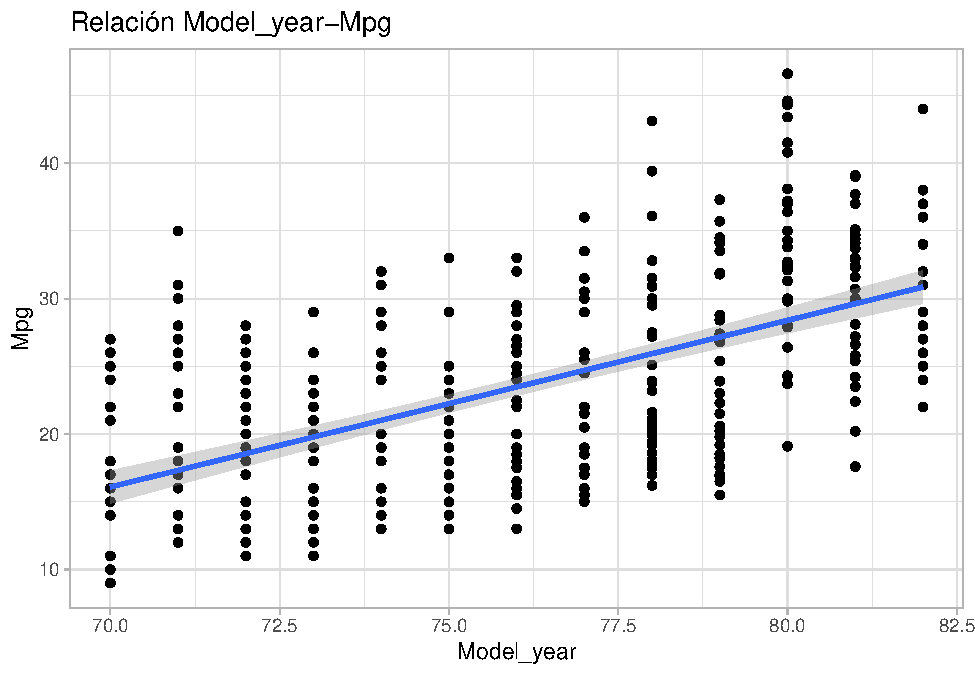
\includegraphics[width=.9\linewidth]{img/EDA_files/figure-latex/unnamed-chunk-32-1} \caption{}\end{figure}

Por desgracia no contamos información sobre los modelos de los coches

Podemos ver como se ubican los diferentes años en un plot Horse\_power vs Mpg

\begin{figure}[H]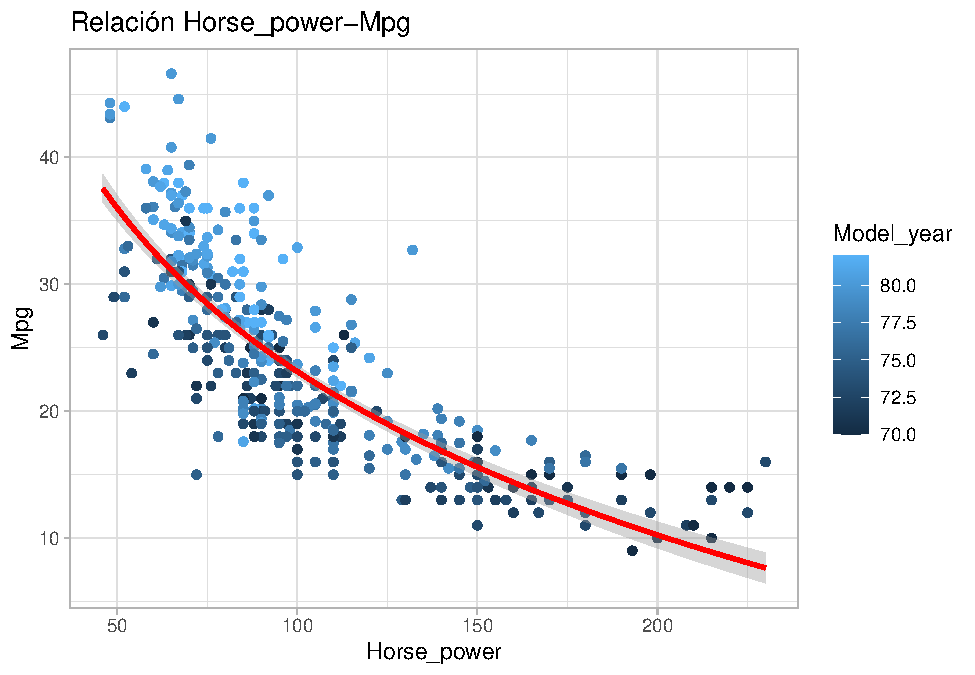
\includegraphics[width=.9\linewidth]{img/EDA_files/figure-latex/unnamed-chunk-33-1} \caption{}\end{figure}

Y vemos que no se puede afirmar la hipótesis, los coches están entremezclados por diferentes años

\begin{itemize}
\item \textbf{H.8}: Esta última hipótesis se puede aplicar al resto de variables, indicándonos que Model\_year no debería tener relevancia para este problema de regresión.
\end{itemize}

No podemos afirmar la hipótesis anterior y por consiguiente esta tampoco.

\begin{itemize}
\item \textbf{H.9}: Horse\_power podría depender de las variables Displacement y Weight
\end{itemize}

Lo hemos comentado anteriormente.

\subsection{Conclusiones}

Como conclusiones podemos decir que tenemos un dataset altamente correlacionado, distribuído de forma no normal pero con la información bien representada. Existen relaciones fuertes entre las variables de entrada y de las de salida para la regresión que probablemente nos ayuden a solucionar con facilidad el problema.

Aunque no hemos descubierto los tipos de distribución que siguen nuestras variables, por si quisiéramos transformarlas a una normal, podemos sin ninguna duda aplicar una estandarización de los datos (puesto que sabemos que no afecta negativamente al problema de regresión) siempre y cuando lo tengamos en cuenta a la hora de analizar los resultados.

Se nos pide elegir 5 regresores para la regresión y contamos exactamente con ese número, por lo que no podemos descartar ninguna variable. Aún así, hemos visto que tenemos algunas variables más interesantes que otras. Variables correladas con la salida nos aumentan las posibilidades de obtener un buen regresor, pero debemos evitar usar variables correladas entre sí para evitar la multicolinealidad. Sería conveniente evitarla para aumentar la interpretabilidad del modelo, pero la potencia en sí de este no cambia. (\url{https://statisticsbyjim.com/regression/multicollinearity-in-regression-analysis/\#}:\textasciitilde:text=Multicollinearity\%20occurs\%20when\%20independent\%20variables,model\%20and\%20interpret\%20the\%20results.) (referenciar esta frase en el apartado de regresión)